%# -*- coding: utf-8-unix -*-
%======================================================================
% qbook.tex for Qbook Template
%======================================================================
% 双面打印
\documentclass{qbook}
\addbibresource{bib/qbook.bib}  % 导入参考文献数据库
\usepackage{indentfirst}
\usepackage{float}
% \usepackage[CJKbookmarks]{hyperref}
\begin{document}
% \pagestyle{empty}
%# -*- coding: utf-8-unix -*-
\thispagestyle{empty}
\begin{tikzpicture}[overlay,remember picture,font=\sffamily\bfseries]
\draw[ultra thick,c4,name path=big arc] ([xshift=-2mm]current page.north) arc(150:285:11)
coordinate[pos=0.225] (x0);
\begin{scope}
\clip ([xshift=-2mm]current page.north) arc(150:285:11) --(current page.north
east);
\fill[c4!50,opacity=0.25] ([xshift=4.55cm]x0) circle (4.55);
\fill[c4!50,opacity=0.25] ([xshift=3.4cm]x0) circle (3.4);
\fill[c4!50,opacity=0.25] ([xshift=2.25cm]x0) circle (2.25);
\draw[ultra thick,c4!50] (x0) arc(-90:30:6.5);
\draw[ultra thick,c4] (x0) arc(90:-30:8.75);
\draw[ultra thick,c4!50,name path=arc1] (x0) arc(90:-90:4.675);
\draw[ultra thick,c4!50] (x0) arc(90:-90:2.875);
\path[name intersections={of=big arc and arc1,by=x1}];
\draw[ultra thick,c4,name path=arc2] (x1) arc(135:-20:4.75);
\draw[ultra thick,c4!50] (x1) arc(135:-20:8.75);
\path[name intersections={of=big arc and arc2,by={aux,x2}}];
\draw[ultra thick,c4!50] (x2) arc(180:50:2.25);
\end{scope} 
\path[decoration={text along path,text color=c4,
	raise = -2.8ex,
	text  along path,
	text = {|\sffamily\bfseries|\today},
	text align = center,
},
decorate
] ([xshift=-2mm]current page.north) arc(150:245:11);
%
\begin{scope}
\path[clip,postaction={fill=c3}]
([xshift=2cm,yshift=-8cm]current page.center) rectangle ++ (4.2,7.7);
\fill[c2] ([xshift=0.5cm,yshift=-8cm]current page.center)
([xshift=0.5cm,yshift=-8cm]current page.center)  arc(180:60:2)
|- ++ (-3,6) --cycle;
\draw[ultra thick,c4] ([xshift=-1.5cm,yshift=-8cm]current page.center) 
arc(180:0:2);
\draw[ultra thick,c4] ([xshift=0.5cm,yshift=-8cm]current page.center) 
arc(180:0:2);
\draw[ultra thick,c4] ([xshift=2.5cm,yshift=-8cm]current page.center) 
arc(180:0:2);
\draw[ultra thick,c4] ([xshift=4.5cm,yshift=-8cm]current page.center) 
arc(180:0:2);
\fill[red] ([xshift=2.5cm,yshift=-8cm]current page.center) +(60:2) circle(1.5mm);
\node[text=c5!80!black] at ([xshift=4.7cm,yshift=-5.2cm]current page.center) {$\rho:=\dfrac{1+\sqrt{-3}}{2}$};
\end{scope}
%
\fill[c1] ([xshift=2cm,yshift=-8cm]current page.center) rectangle ++ (-13.7,7.7);
\node[text=white,anchor=west,scale=4,inner sep=0pt] at
([xshift=-10.55cm,yshift=-3cm]current page.center) {场景文字处理};
\node[text=white,anchor=west,scale=2,inner sep=0pt] at
([xshift=-4.5cm,yshift=-5.5cm]current page.center) {华中科技大学};
\end{tikzpicture}  % 载入封面
% \begin{center}
% 	\Large{\sffamily\bfseries\heiti Version 2.00} \\ \vspace{2em}
% 	\Large{\sffamily\bfseries\heiti 编译日期: \today} \\ \vspace{1em}
% 	\Large{\sffamily\bfseries\heiti 任何建议及错误信息请发送至邮箱} \\
% 	\texttt{jey74165@163.com}
% \end{center} 
% \vfill
% \vspace{30em}
% \begin{tabular*}{\textwidth}{ccc}
% 	\includegraphics{figure/by-nc.eps}
% 	& \begin{minipage}[b]{0.6\textwidth}
% 		\small\sffamily
% 		本作品采用知识共享 署名-非商业性使用 4.0 国际 许可协议进行许可. 访问\url{http://creativecommons.org/licenses/by-nc/4.0/  }查看该许可协议.
% 	\end{minipage}
% \end{tabular*}  
% \thispagestyle{empty}
% \frontmatter  % 对前言和概览用罗马数字作为页码
% \pagestyle{empty}
% 
\begin{pre}
	\thispagestyle{empty}
	\begin{center}
		{\kaishu{人在春风和气中}}
	\end{center}

\vspace*{5\baselineskip}
\centerline{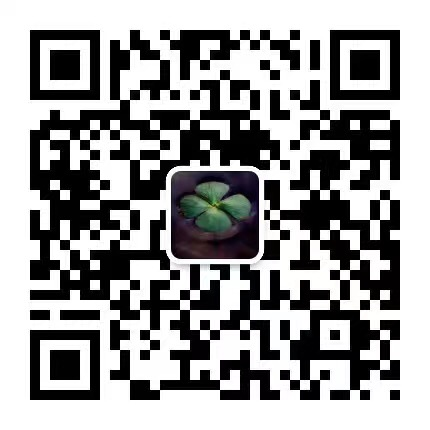
\includegraphics[scale=0.6]{example/gzh.jpg}}
\centerline{\fontsize{26pt}{26pt} 微信公众号}
\end{pre}
% \pagestyle{empty}

\tableofcontents
% \cleardoublepage
\let\cleardoublepage\clearpage
% %# -*- coding: utf-8-unix -*-
\begin{overview}
\thispagestyle{empty}
在2018年3月底,翻译\footnote{这个模板原本是用于一项书籍翻译计划的,关注我公众号的读者对此有所了解。然而由于版权原因,该译本无法公开分享。}进度已过大半,于是开始着手进行\LaTeX 排版。在此之前我对\LaTeX 的了解微乎其微,甚至第一次安装TexLive就出了问题,不得不重新安装。也是借着给这个译本排版的机会,才逐渐熟悉了这一软件的使用方法。

如大家所见,模板的封面和扉页设计均高仿\footnote{李老师的书籍源码尚未公开,此为仿作。}自李文威老师《模形式初步》一书,并已得到李老师的使用许可;定理和定义环境则取材自网上流传的Elegantbook模版。我也从这一以模仿为主的学习过程中,对\LaTeX 有了更深入的了解。

本模板命名为$\mathbb{ Q }$-book,谐音自cubic一词。由于是一个菜鸟的作品,自然还有许多瑕疵,对此模板的错误和不足之处还请各位多多包涵。

\end{overview}
 
\mainmatter	  % 对正文用阿拉伯数字作为页码
%======================================================================
% 正文内容
\pagestyle{fancy}
% \setcounter{page}{0}

%# -*- coding: utf-8-unix -*-
%%==================================================
\chapter{文字识别(Scene Text Recognition)}
\cite{scatter,2020srn,wan2019textscanner}
\section{文字识别方法介绍}
\subsection{DAN}
DAN\cite{wang2019decoupled}的主要是解决基于attention机制的识别器中因需要依赖先前预测结果(存在错误累积)所导致的注意力不对齐的问题。
文章中通过解耦注意力机制和语义模型来解决该问题。解耦过程如图\ref{dan_introduction}所示。
\begin{figure}[H]
    \centering
    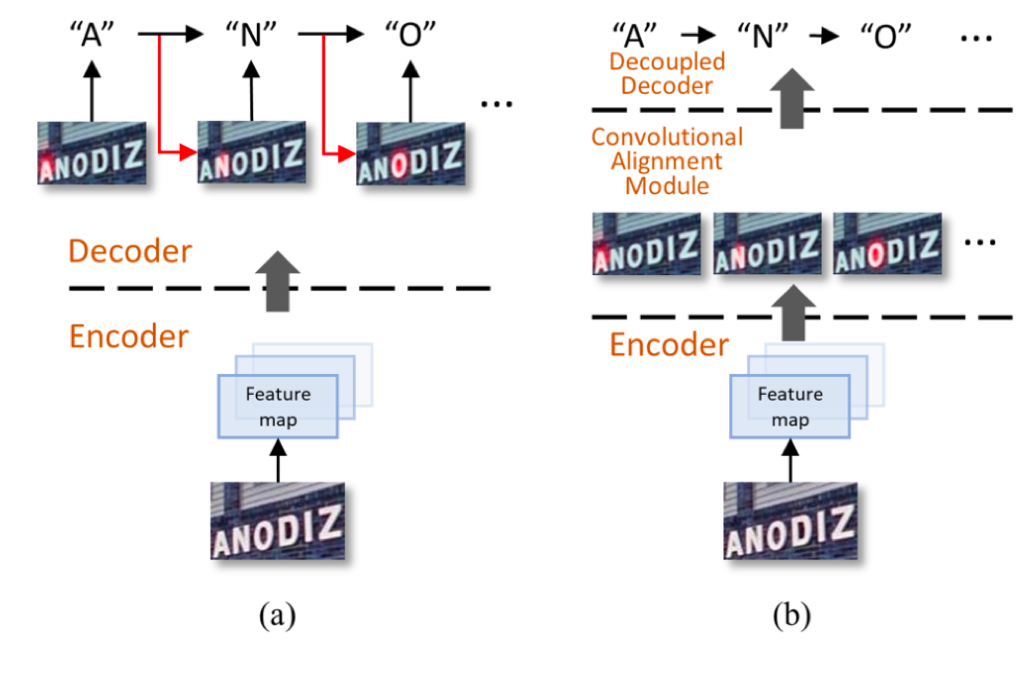
\includegraphics[width=.7\textwidth]{figure/recognition/dan_introduction.png} 
    \caption{DAN解耦过程:(a)之前的基于注意力机制的方法将注意力模块和语义推理模块放在一起;(b)DAN
    中先预测注意力,然后进行语义模块的预测。} 
    \label{dan_introduction} 
\end{figure}

\subsubsection{DAN的网络结构}
DAN的网络结构如图\ref{dan_framework}所示:Decoupled Text Decoder是基于GRU的,其过程和其他文字识别器的一致;
CAM用于预测每一步的attention map。
\begin{figure}[H]
    \centering
    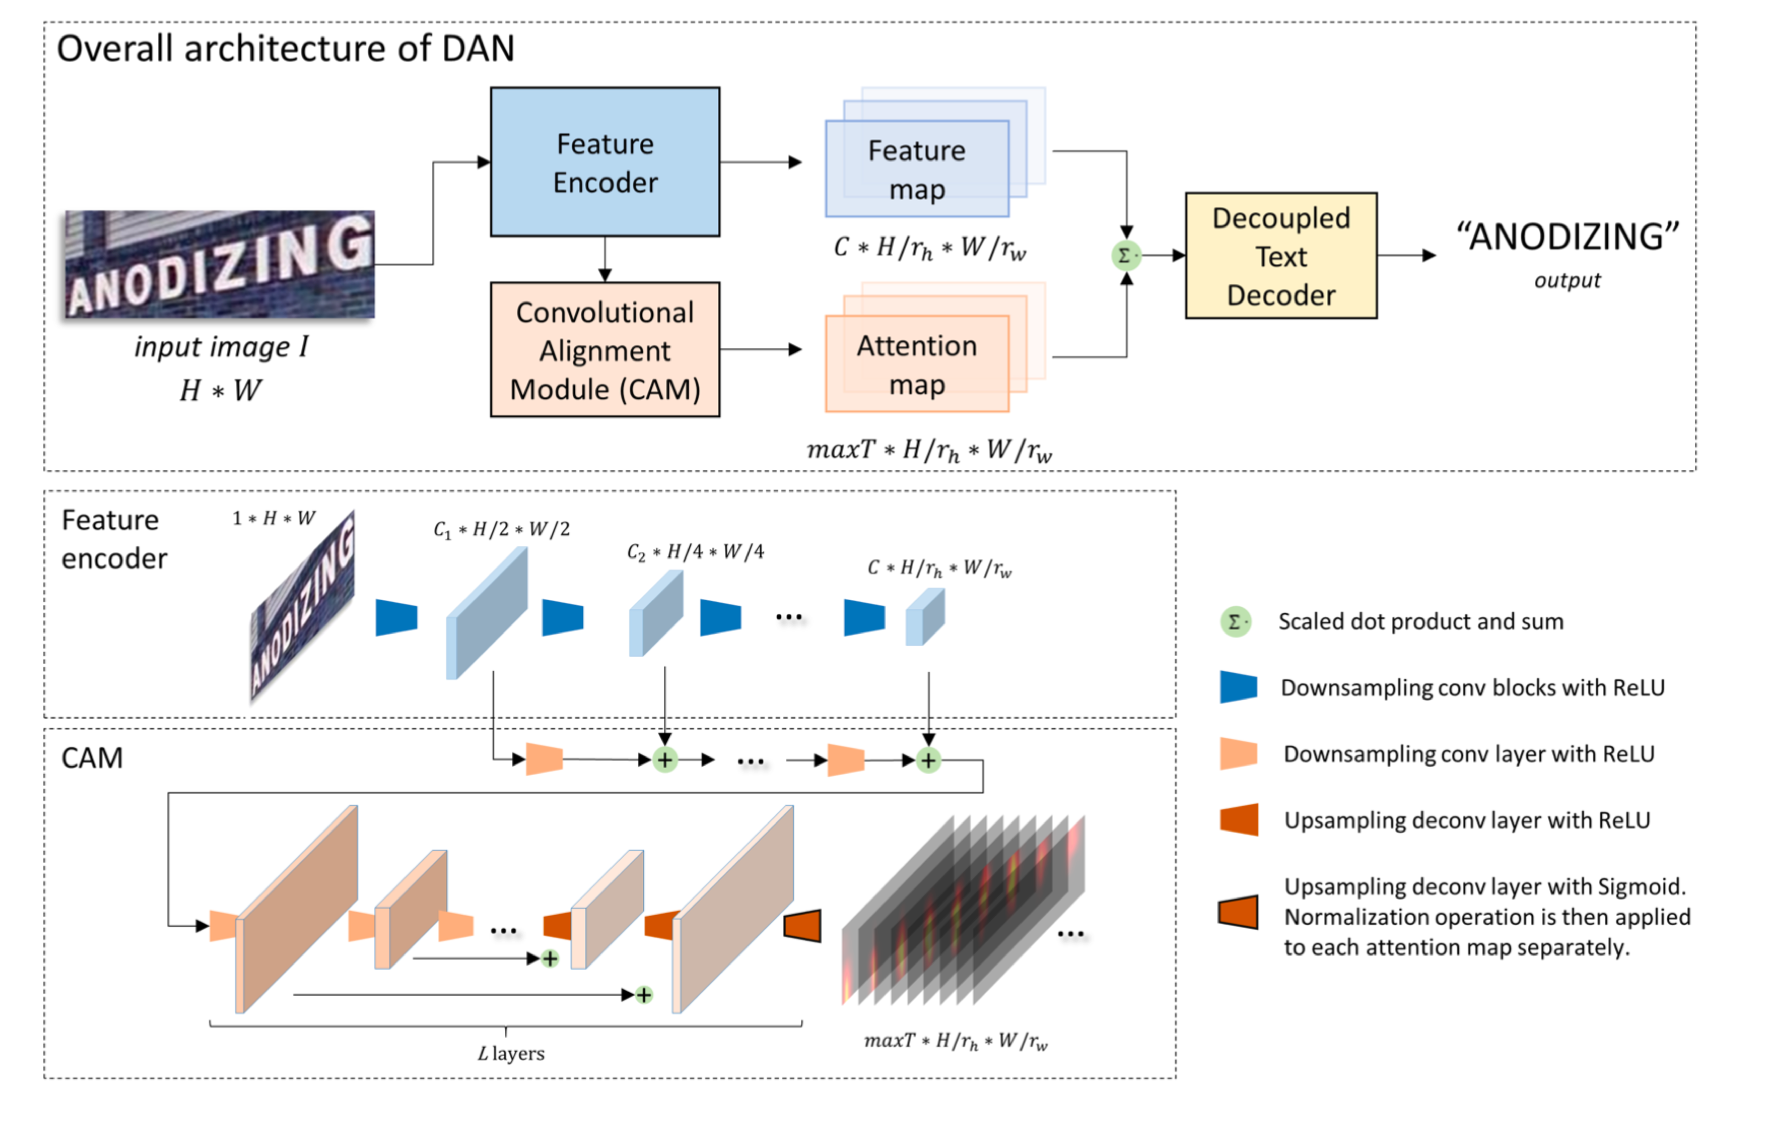
\includegraphics[width=.9\textwidth]{figure/recognition/dan_framework.png} 
    \caption{DAN网络结构。} 
    \label{dan_framework} 
\end{figure}

\subsection{GTC}
GTC\cite{hu2020gtc}的主要是解决基于CTC的文字识别器中帧数不对齐的问题,比如字符'H'由于分帧的原因会被识别为'I'。
文章中通过基于注意力机制的识别head的监督来使得特征在一定程度上对齐。在测试阶段为了保证效率,只使用基于CTC的识别head。
另外,CNN特征经过分帧后,相邻帧之间在视觉上具有一定的相似性,为了使得特征能够进一步对齐(理想情况下一帧的特征代表一个字符的特征),
作者使用GCN来建模帧之间的关系,融合后得到对齐的帧。
\begin{figure}[H]
    \centering
    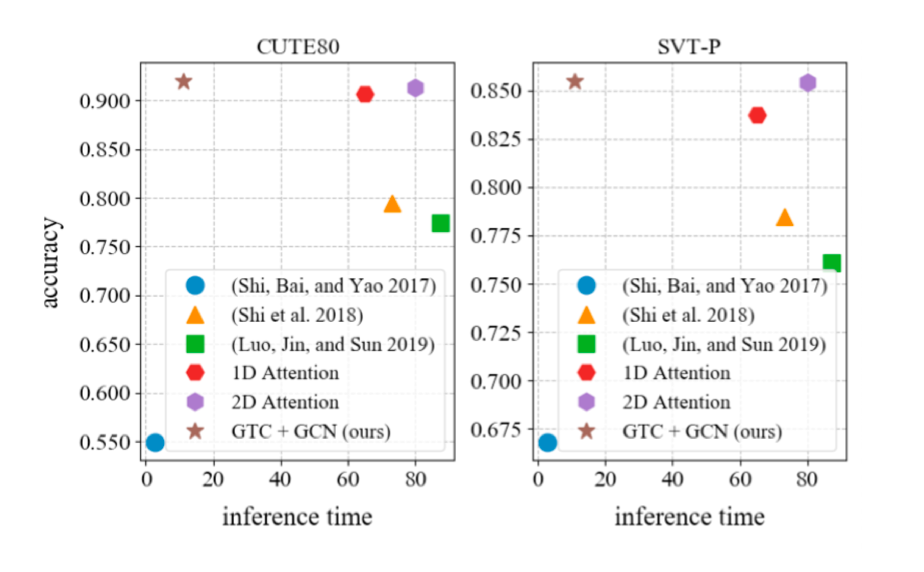
\includegraphics[width=.8\textwidth]{figure/recognition/gtc_introduction.png} 
    \caption{GTC准确率和效率的关系,x轴代表ms/image} 
    \label{gtc_introduction} 
\end{figure}

\subsubsection{GTC的网络结构}
GTC的网络结构如图\ref{gtc_framework}所示:网络的整体结构和Aster类似,不同的是,识别的head是基于CTC的,基于注意力机制的识别head在训练时
起到辅助作用,使得特征能够起到一定的对齐作用。为保证效率,测试过程只使用CTC进行解码,最终的精度-效率对比如图\ref{gtc_introduction}所示。
\begin{figure}[H]
    \centering
    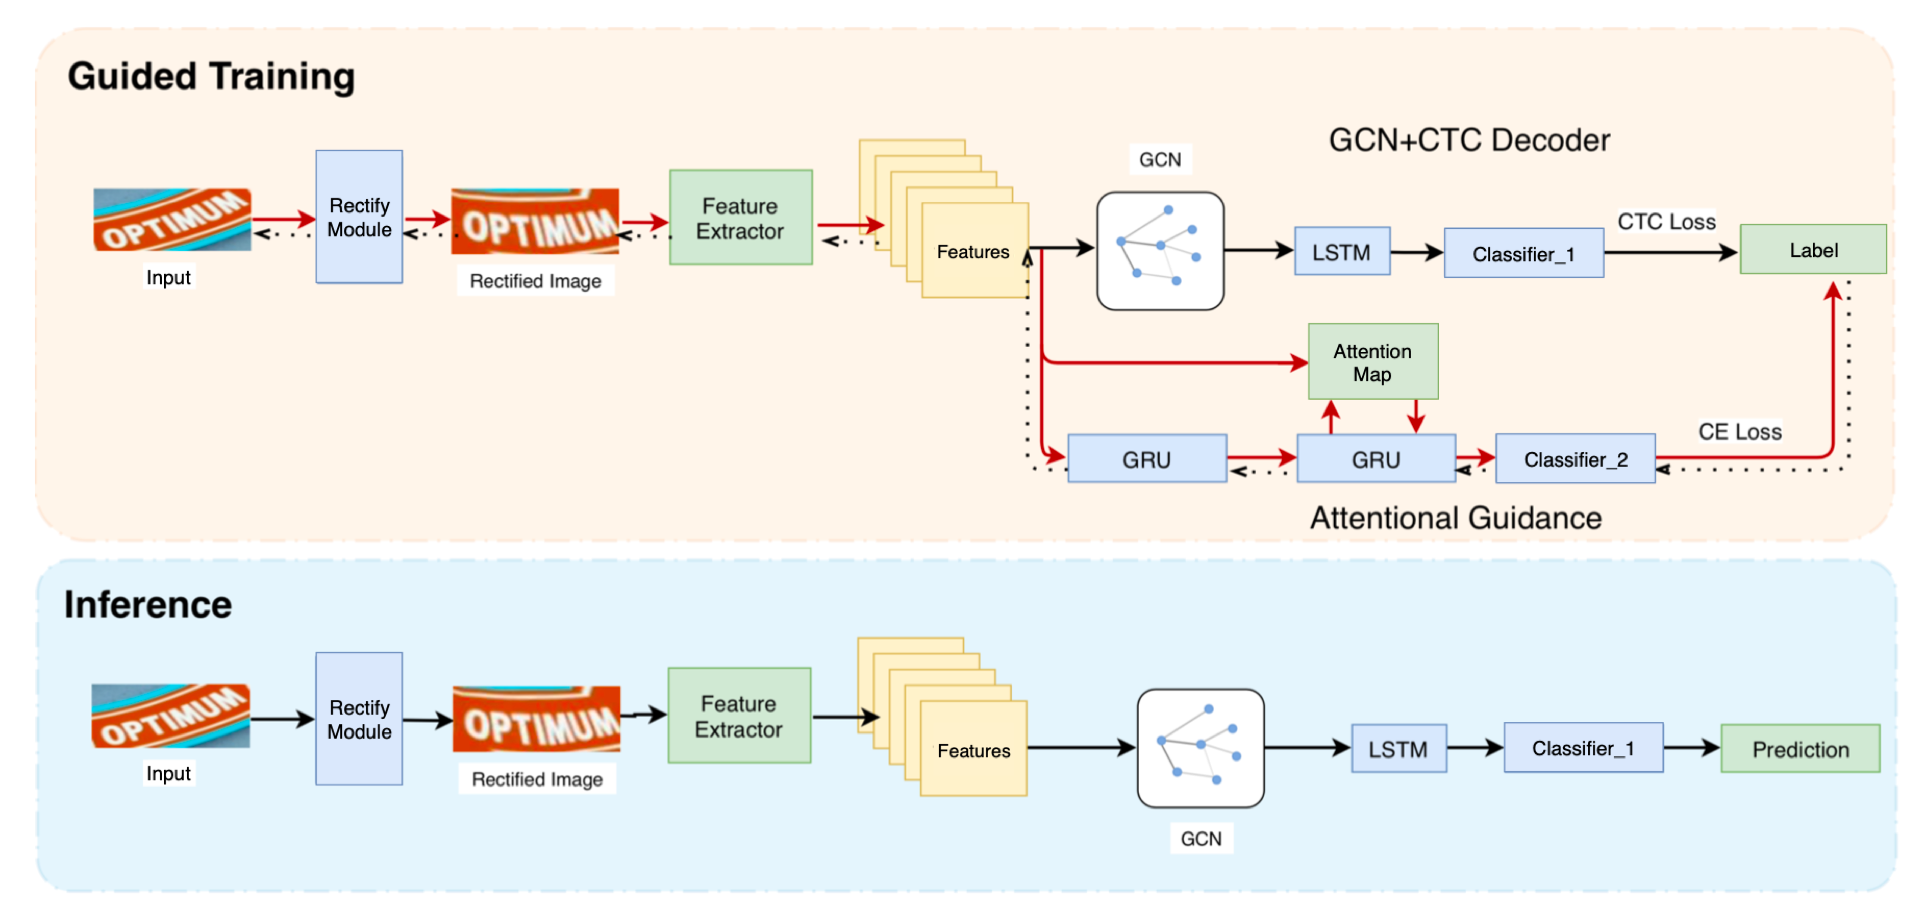
\includegraphics[width=.98\textwidth]{figure/recognition/gtc_framework.png} 
    \caption{GTC网络结构。} 
    \label{gtc_framework} 
\end{figure}


\subsection{TextScanner}
TextScanner\cite{wan2019textscanner}的主要是解决基于分割的文本识别器中字符分割不准以及基于注意力机制的文本识别器中注意力发散的问题。目的仍然是
寻找精准的字符定位从而使得特征对齐。如图\ref{textscanner_introduction}:基于注意力机制和分割的方法对字符的定位都存在一些问题,文章中通过预测单词
的阅读顺序来解决该问题。

\begin{figure}[H]
    \centering
    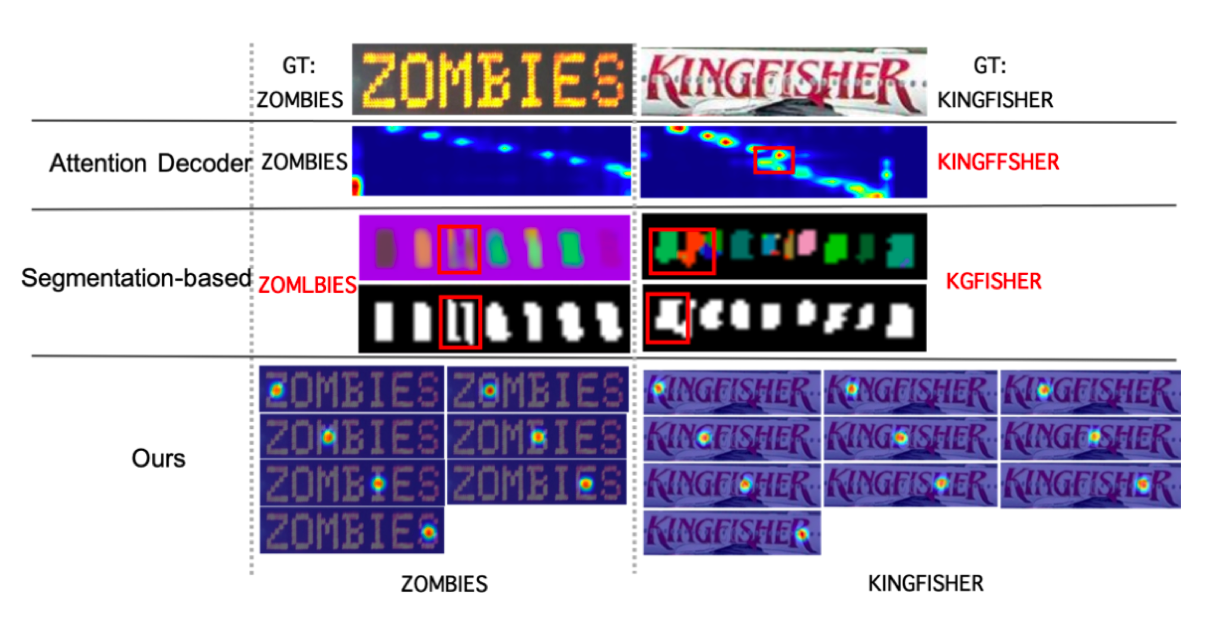
\includegraphics[width=.8\textwidth]{figure/recognition/textscanner_introduction.png} 
    \caption{TextScanner问题出发点:Attention Decoder中注意力容易发散;基于分割的方法中因为阈值问题,容易存在欠分割或过分割问题。} 
    \label{textscanner_introduction} 
\end{figure}

\subsubsection{TextScanner的网络结构}
TextScanner的网络结构如图\ref{scatter_framework}所示:整体分为三部分,1)字符分割模块,每个像素对类别进行预测;2)字符顺序分割模块,其中N代表
最大长度,模块进行N分类,预测每个像素属于哪一时间时刻;3)字符定位模块用于定位每个字符。
\begin{figure}[H]
    \centering
    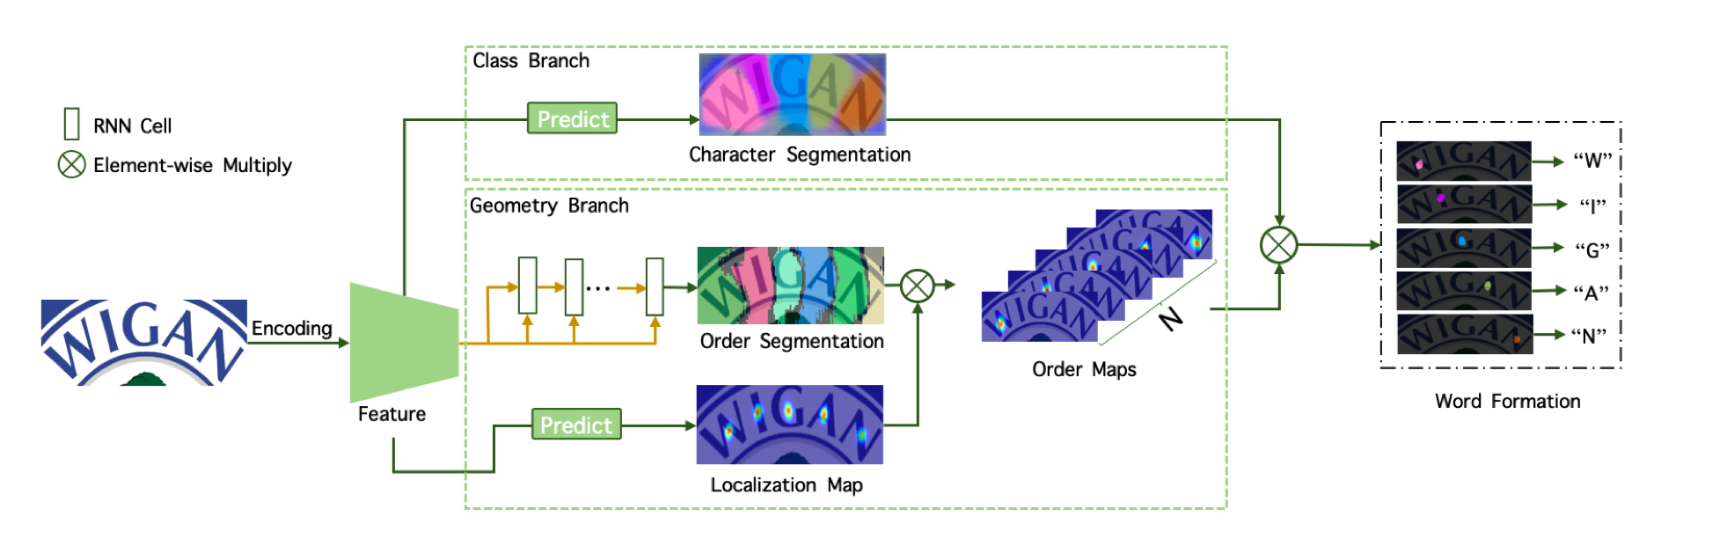
\includegraphics[width=.98\textwidth]{figure/recognition/textscanner_framework.png} 
    \caption{TextScanner网络结构。} 
    \label{textscanner_framework} 
\end{figure}

\subsection{SCATTER}
SCATTER\cite{scatter}的主要研究目的是让网络不断迭代地选择图像的视觉特征(CNN的特征)和语义特征(RNN建模出的语义特征)来强化
模型的特征提取能力。而特征选择的过程通过注意力机制来完成。
\subsubsection{SCATTER的网络结构}
SCATTER的网络结构如图\ref{scatter_framework}所示,网络的整体框架和Aster一致,不同之处在于:SCATTER在Visual features
和Contextual features之间加入了多层特征选择模块进行特征的优化,并且在Visual features中加入了CTC进行监督学习。特征选择模块
网络结构如图\ref{scatter_feature_select}所示。
\begin{figure}[H]
    \centering
    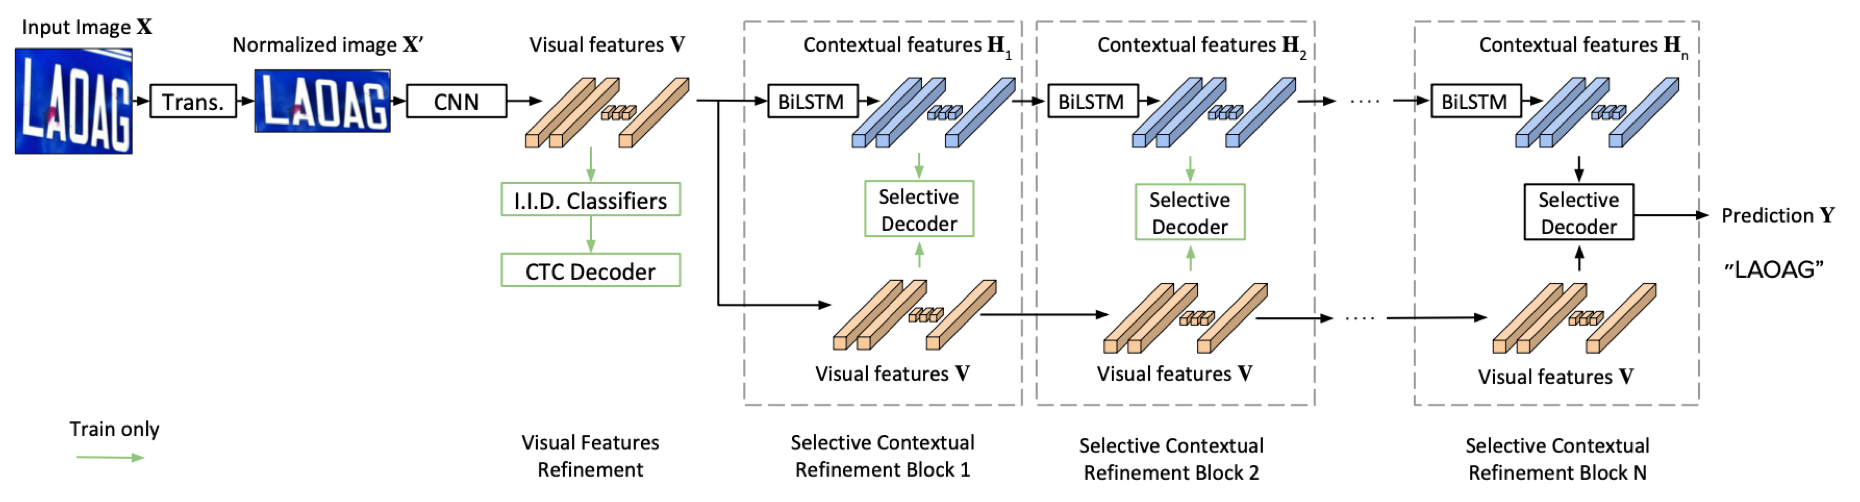
\includegraphics[width=.98\textwidth]{figure/recognition/scatter_framework.png} 
    \caption{SCATTER网络结构。} 
    \label{scatter_framework} 
\end{figure}

\begin{figure}[H]
    \centering
    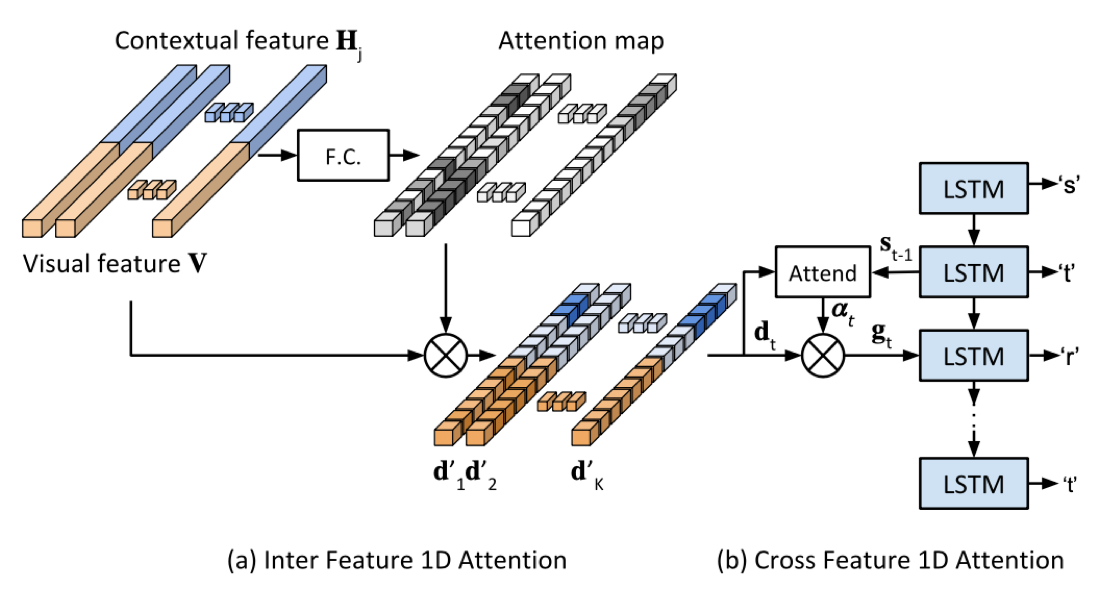
\includegraphics[width=.8\textwidth]{figure/recognition/scatter_feature_select.png} 
    \caption{SCATTER特征选择模块。} 
    \label{scatter_feature_select} 
\end{figure}

\subsection{SRN}
SRN的主要出发点是:
1)在文字识别中,由于光照,旋转等因素的影响,仅仅依靠图像的视觉特征
极易引起单词中某个字符预测错误。对于这些易错的字符,如果能够利用单词的语义信息,那么
将会极大地降低该字符的预测错误率。如图\ref{srn_introduction}所示,如果仅仅观察每个字符的视觉特征(b),
某些字符容易预测错误,结合上下文语义信息能够缓解因视觉特征混淆而引起的错误预测。
2)文字识别中基于注意力机制的识别器中\cite{shi2018aster},注意力模块的输出大多是串行的,注意力模块中当前时刻
的预测非常依赖于前一时刻的输出,导致模型难以并行处理。为解决模型的效率问题,提出并行的注意力模块。


\begin{figure}[H]
    \centering
    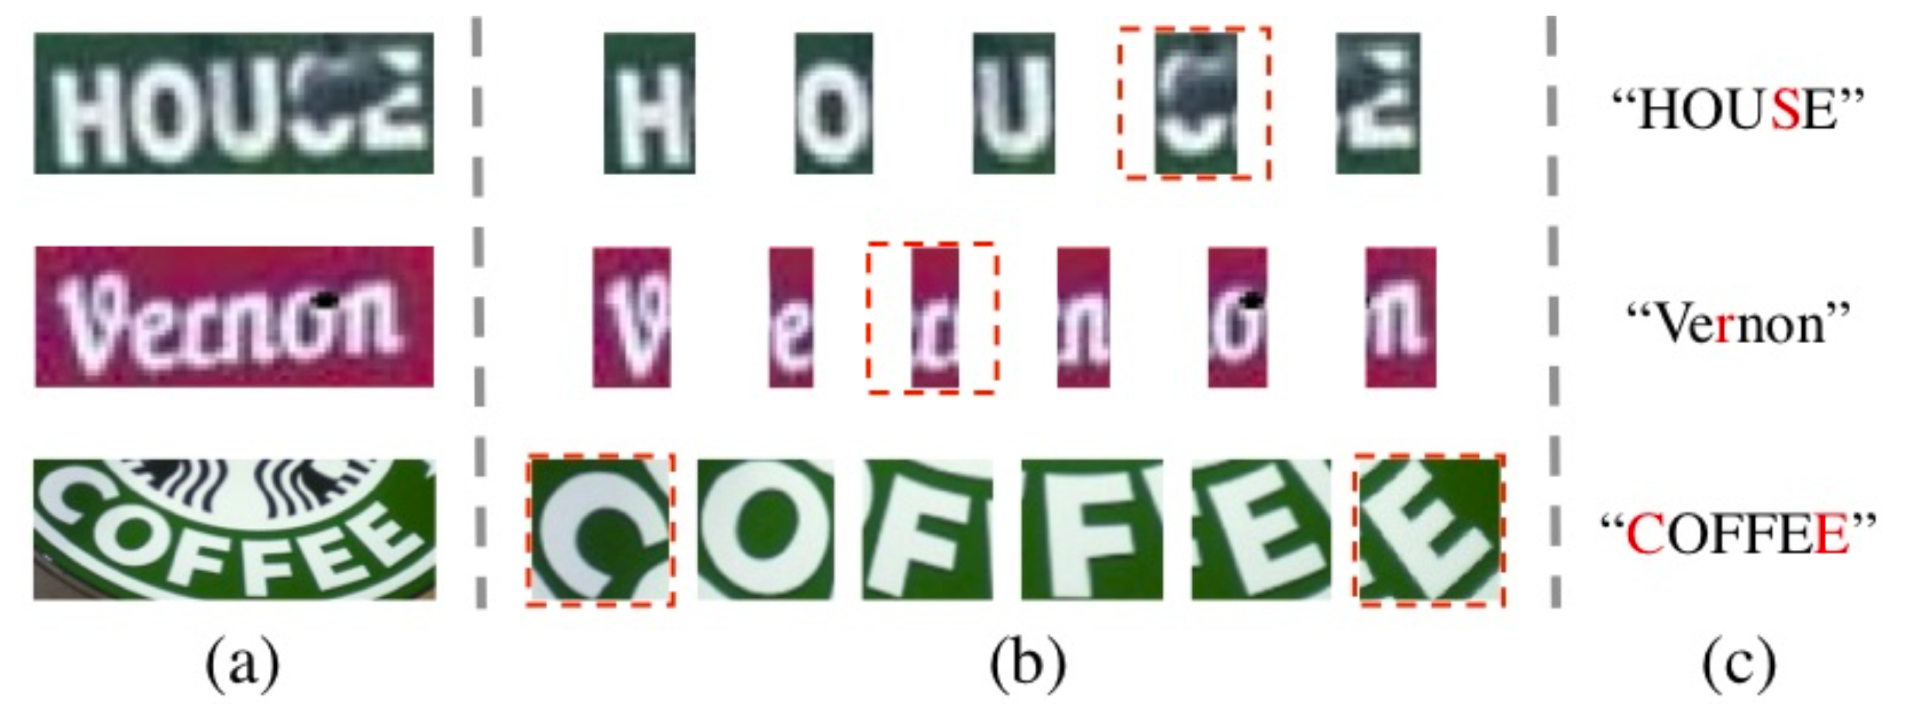
\includegraphics[width=.8\textwidth]{figure/recognition/srn_introduction.png} 
    \caption{单词中容易预测错误的字符案例:(a)表示原图;(b)表示字符,红色标注为易错字符;(c)为利用上下文语义信息预测结果。} 
    \label{srn_introduction} 
\end{figure}

\subsubsection{SRN的网络结构}
SRN的网络结构如图\ref{srn_framework}所示:1)整体网络的backbone为FPN网络,用于提取图像的视觉特征;2)并行的视觉注意力模块(PAVM)用于定位每个字符;3)全局的语义推理模块(GSRM)
用于利用语义上下文来预测字符。
\begin{figure}[H]
    \centering
    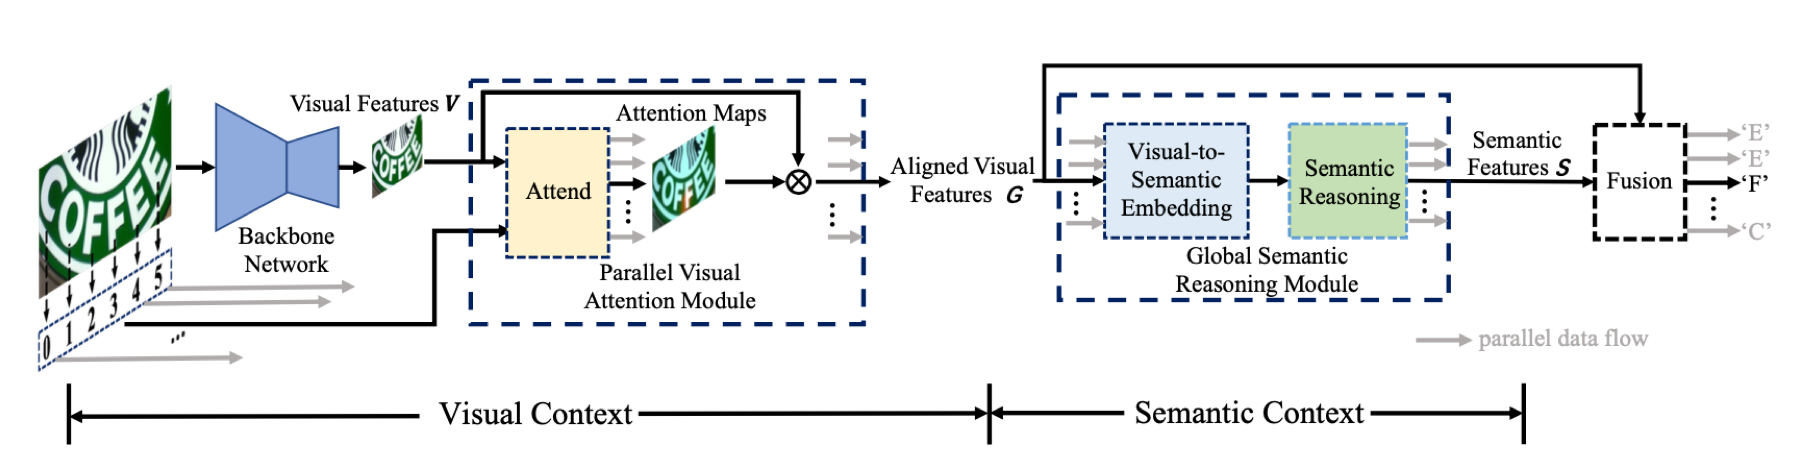
\includegraphics[width=.98\textwidth]{figure/recognition/srn_framework.png} 
    \caption{SRN网络框架图。} 
    \label{srn_framework} 
\end{figure}

\begin{figure}[H]
    \centering
    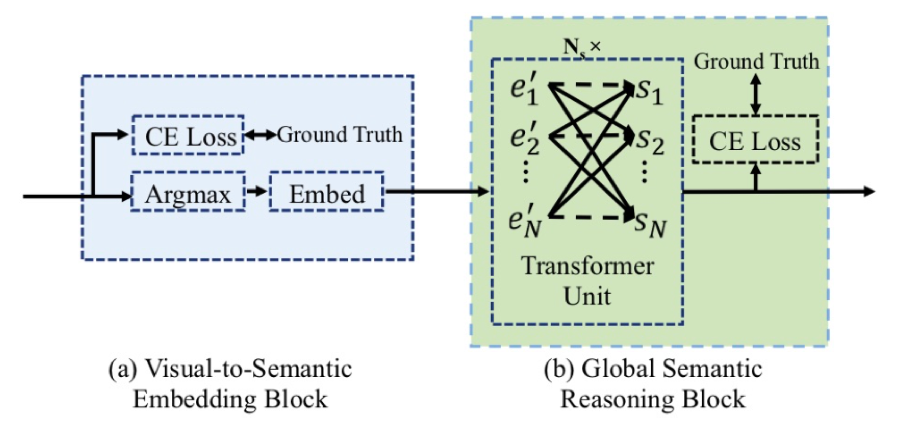
\includegraphics[width=.8\textwidth]{figure/recognition/srn_gsrm.png} 
    \caption{GSRM模块结构。} 
    \label{srn_gsrm} 
\end{figure}
\subsubsection{SRN并行以及语义推理分析}
SRN的主要优势在于利用单词的上下语义来预测困难字符,而要实现这一特性的技术难点却在于如何并行化处理序列预测。
因为在预测t时刻的字符时,需要其他所有时刻的特征。因此,SRN中如何将各个模块并行化是该方法技术的重点。
表\ref{srn_process}详细地对比了SRN中并行化与Aster中串行化的区别。

对于并行化处理方面,SRN的主要改进在于两大方面:1)将注意力模型并行化。传统的注意力模型
依赖于前一时刻的隐藏状态$h_{t-1}$(在注意力模块中,$h_{t-1}$作为key来获取相似度)从而无法并行化。SRN中将
传统注意力模型中的key改为$O_{t}$(代表字符顺序,第一个字符为0,第二个字符为1)的Embedding特征,从而实现并行化;
2)将语义模型并行化。先前的文字识别算法中利用rnn来对文字语义进行建模,而rnn中以前一时刻的预测结果的Embedding特征
$f_{y}(y_{t-1})$作为输入,从而无法并行化。SRN中将$e_{t}^{'}$(以$g_{t}$为输入的预测结果的Embedding向量)来代替,
从而实现并行化。另外,通过Transformer Unit来获取多路径的语义信息,能够考虑当前时刻的前向以及后向的所有语义信息。
\begin{table}[!htbp]
    \centering
    \caption{SRN中PVAM,GSRM模块和Aster的串行注意力机制与串行语义模块的区别。其中TU为Transformer Unit,
    $v_{i}$为视觉特征,$h_{i}$为隐藏状态,$y_{t}$为字符label,$O_{t}$为阅读顺序。} 
    \begin{tabular}{|c|l|l|}
    \hline 
    Module&Aster&SRN\\
    \hline 
    \multirow{3}*{Attention}&
    $e_{t,i}=W^{T}_{e}tanh(W_{h}h_{t-1} + W_{v}v_{i})$& 
    $e_{t,i}=W^{T}_{e}tanh(W_{o}f_{o}(O_{t}) + W_{v}v_{i})$\\
    &$\alpha_{t,i}=exp(e_{t,i})/\sum_{i^{'}=1}^{n}exp(e_{t,i^{'}})$&
    $\alpha_{t,i}=exp(e_{t,i})/\sum_{i^{'}=1}^{n}exp(e_{t,i^{'}})$\\
    &$g_{t}=\sum_{i=1}^{n}\alpha_{t,i}v_{i}$&
    $g_{t}=\sum_{i=1}^{n}\alpha_{t,i}v_{i}$\\
    \hline 
    \multirow{2}*{Semantic Reasoning}&
    \multirow{2}*{$(x_{t}, h_{t}) = rnn(h_{t-1}, (g_{t}, f_{y}(y_{t-1})))$}&
    $e_{t}^{'} = f_{e}(softmax(f_{g}(g_{t})))$\\
    &&$s_{t} = TU(e_{0}^{'}...e_{t-1}^{'}e_{t+1}^{'}...e_{n}^{'})$\\
    \hline 
    \multirow{2}*{Fusion}&&$z_{t} = sigmoid(W_{z}[g_{t},s_{t}])$\\
    &&$f_{t} = z_{t}g_{t} + (1-z_{t})s_{t}$\\
    \hline 
    Classification&
    $p(y_{t}) = softmax(Wx_{t}+b)$&
    $p(y_{t}) = softmax(Wf_{t}+b)$\\
    \hline
    \end{tabular}
    \label{srn_process} 
\end{table}

\begin{figure}[H]
    \centering
    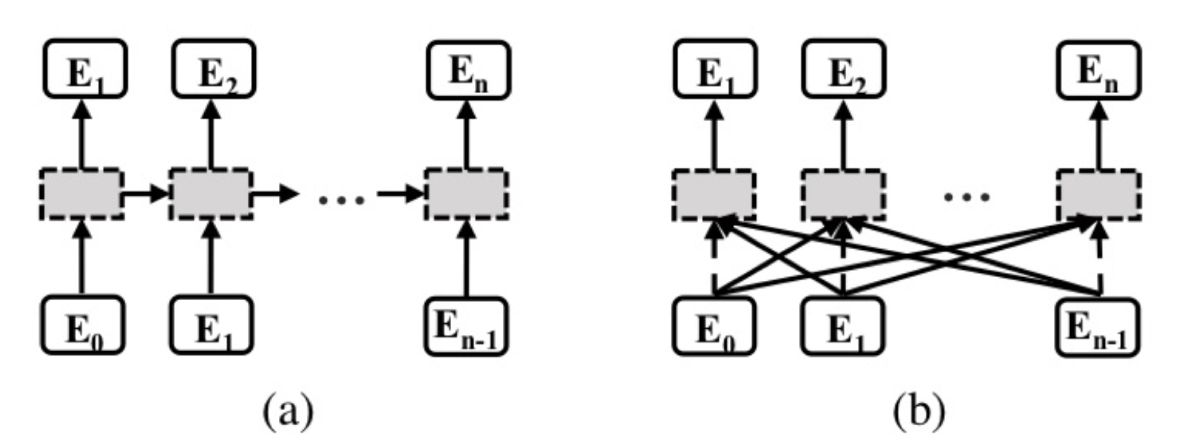
\includegraphics[width=.98\textwidth]{figure/recognition/srn_multiway.png} 
    \caption{a)rnn中建模单词语义模型;b)SRN中建模单词语义模型能够考虑各个路径的信息,避免单向的错误累积。} 
    \label{srn_multiway} 
\end{figure}

\subsection{SEED}
Not Publication
%# -*- coding: utf-8-unix -*-
%%==================================================
\chapter{文字检测(Scene Text Detection)}

\section{文字检测是什么?}

\section{基于回归的方法}

\section{基于分割的方法}


\section{其他方法}

%# -*- coding: utf-8-unix -*-
%%==================================================
% \addbibresource{bib/qbook.bib}
\chapter{端到端文字识别(Scene Text Spotting)}


2018年以前,关于Scene Text Spotting的论文\cite{liu2018fots},主要集中在解决旋转文本的端到端识别问题,几乎没有论文解决曲形文本端到端识别的问题。
自从发表在ECCV2018中的论文,MaskTextSpotter\cite{lyu2018mask},开始试图解决曲形文本端到端识别的问题以来,大量的工作开始致力于该问题的研究,如
\cite{lyu2018mask,liao2019mask,Feng_2019_ICCV,Xing_2019_ICCV,qin2019towards,wang2019all,liu2020abcnet,qiao2020text}。自此,
端到端文本识别方法在理论上能够解决任意形状文本识别的问题。在以下表述中以“任意形状文本端到端识别方法”来统称既能处理多方向又能处理曲形文本的端到端文本识别
方法。

\begin{figure}[H]
    \centering
    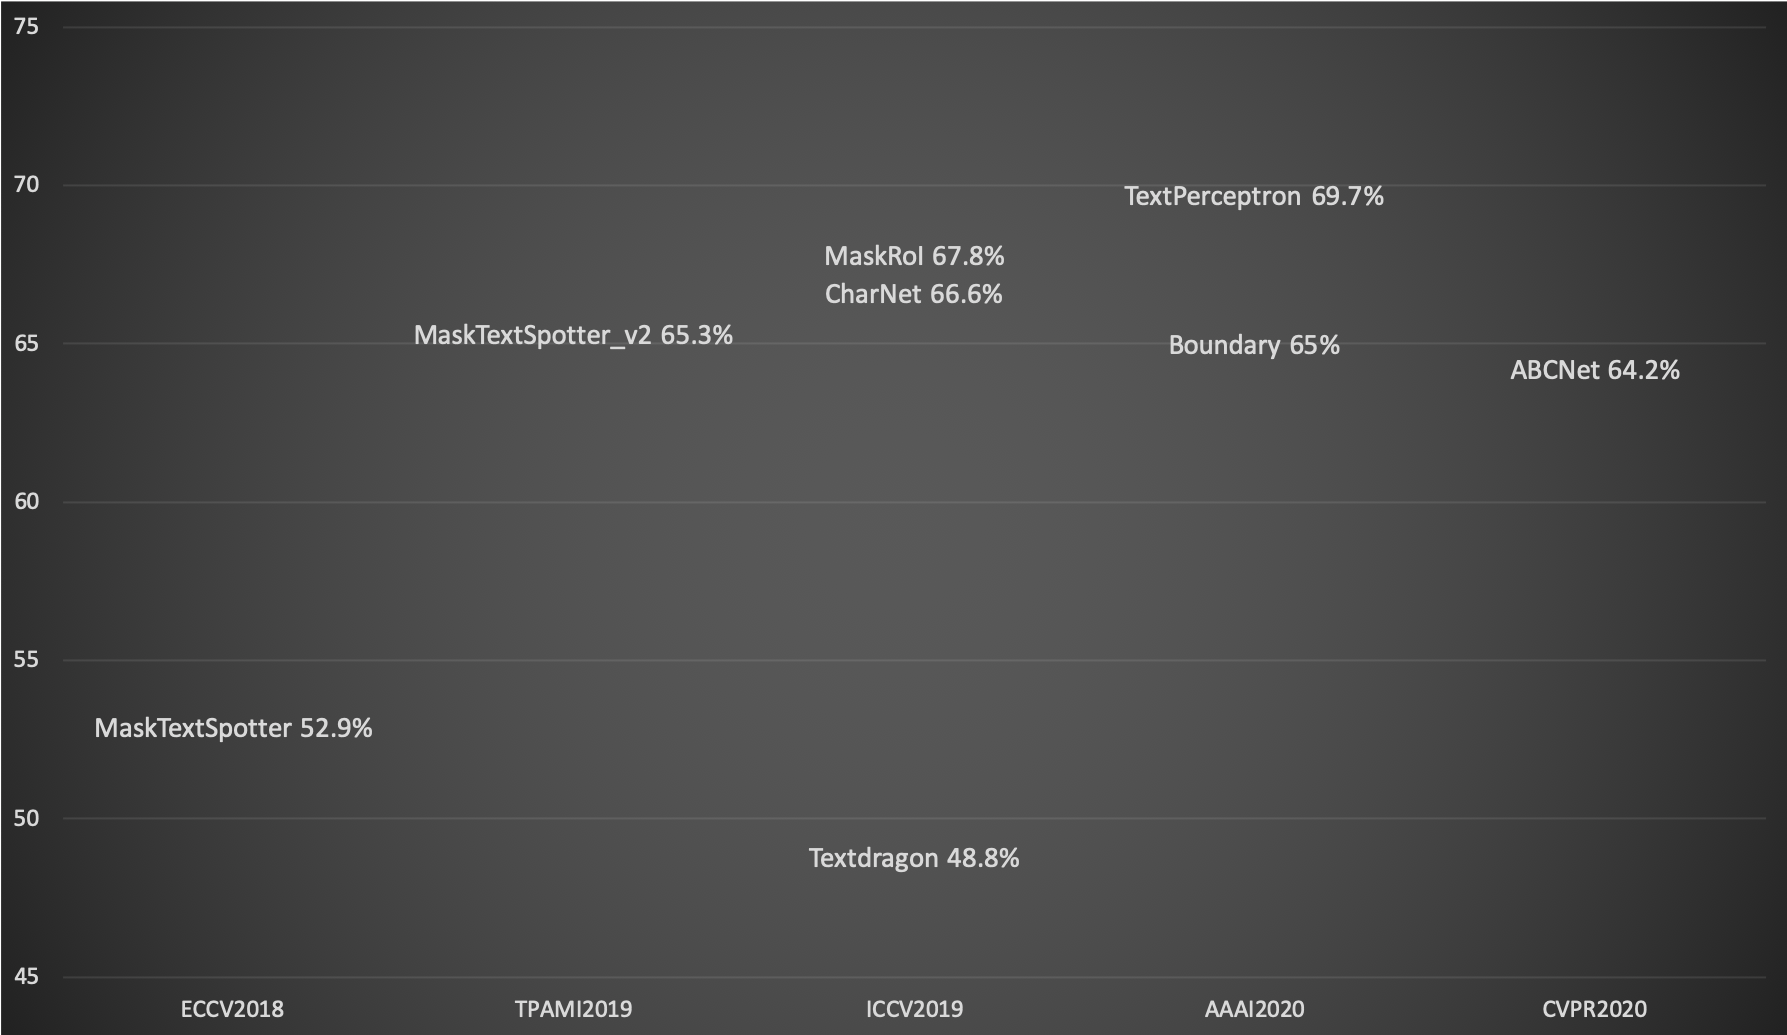
\includegraphics[width=.98\textwidth]{figure/spotting/trends.png} 
    \caption{2018年到2020年3月期间,曲形文本端到端文本识别方法汇总。} 
    \label{spotting_tends} 
\end{figure}

首先,我们从问题的角度出发,概述各种任意形状文本端到端识别方法之间的关系。然后将从方法,实验结果,该方法的优缺点等方面来分别探讨各种方法,这些方法包括:
MaskTextSpotter\cite{lyu2018mask,liao2019mask}、TextDragon\cite{Feng_2019_ICCV}、CharNet\cite{Xing_2019_ICCV}、
MaskRoI\cite{qin2019towards}、Boundary\cite{wang2019all}、TextPerceptron\cite{qiao2020text}以及ABCNet\cite{liu2020abcnet}。
最后,进一步总结归纳以上方法的特点。



\section{任意形状文本端到端识别方法的发展脉络}



\section{各种任意形状文本端到端识别方法介绍}
\subsection{MaskTextSpotter}
\subsubsection{MaskTextSpotter网络结构}
MaskTextSpotter作为首个任意形状文本端到端识别方法,其思路是将每个文字字符作为一个类别进行检测。其网络框架如图\ref{masktextspotter_framework}所示,网络
主体部分与MaskRCNN\cite{he2017mask}一致。由于常规的MaskRCNN网络(分割分支进行1通道的分割,表示是否为文字两个类别)只能完成文字检测任务,无法进行文字识别,
因此作者将Mask分支设计为37个通道(26个英文字符加上10个数字以及表示是否为字符区域的1通道)加上检测的1个类别共38个类别进行分割,其分割分支如图\ref{masktextspotter_maskbranch}所示。
在测试阶段,检测的1通道能够检测任意形状的文本。根据另外37个通道的分割信息,按照从左到右的顺序连接每个字符,完成识别任务。

\begin{figure}[htb]
    \centering
    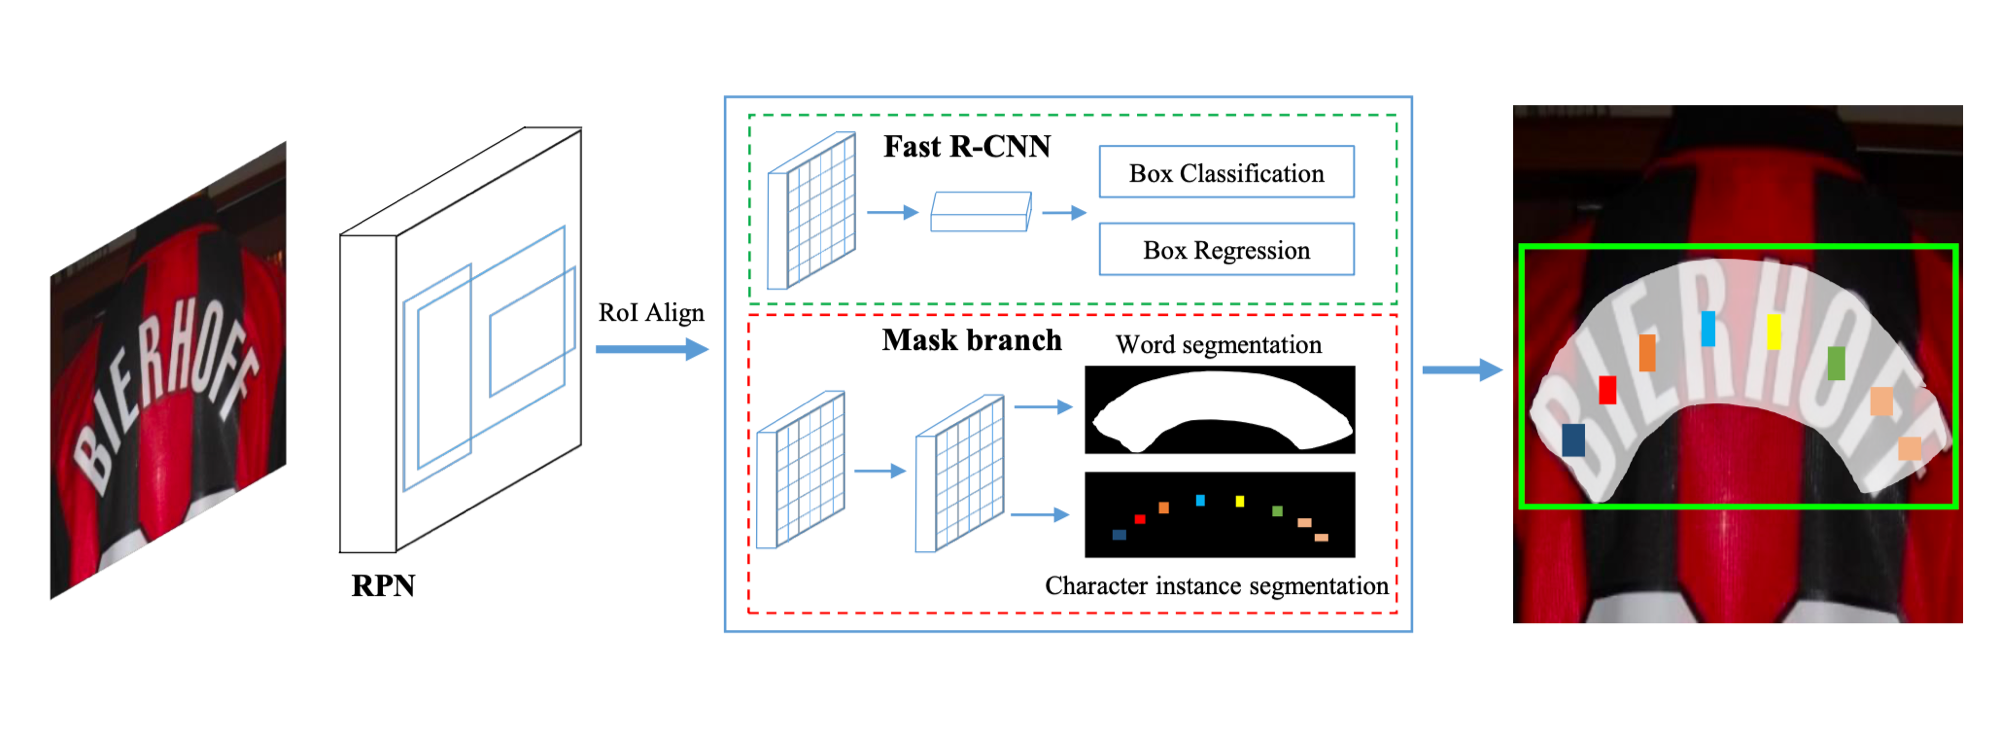
\includegraphics[width=.98\textwidth]{figure/spotting/masktextspotter_framework.png} 
    \caption{MaskTextSpotter框架图。} 
    \label{masktextspotter_framework} 
\end{figure}

\begin{figure}[htb]
    \centering
    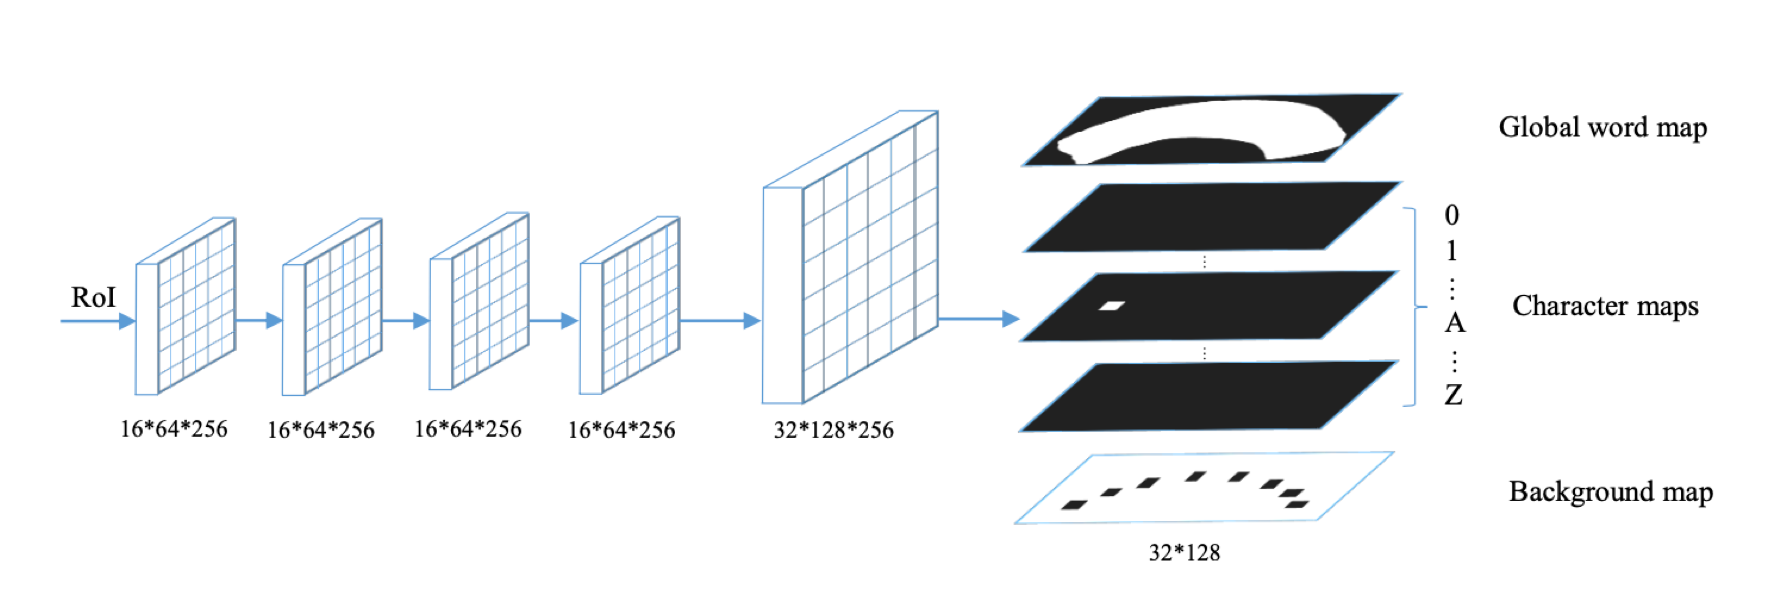
\includegraphics[width=.98\textwidth]{figure/spotting/masktextspotter_maskbranch.png} 
    \caption{MaskTextSpotter的分割分支结构图。} 
    \label{masktextspotter_maskbranch} 
\end{figure}

\subsubsection{MaskTextSpotter实验细节}
MaskTextSpotter的训练过程分为两部分:合成数据集预训练和真实数据集微调阶段。合成数据集使用的是SynthText\cite{gupta2016synthetic},batch size为8,输入图像
以短边为800,保持长宽比进行训练。在真实数据微调阶段,batch size为8,采用多尺度训练的策略,短边分为(600,800,1000)三个尺度进行训练,
使用的数据集有SynthText, ICDAR2013, ICDAR2015, TotalText以及来自\cite{zhong2016deeptext}的1162张图像。

\subsubsection{MaskTextSpotter\_v2网络结构}
由于MaskrTextSpotter中将通过将每个字符作为单独的类别分割出来作为识别结果,这样会导致识别过程中忽略文字的语义特征。基于此,MaskTextSpotter\_v2的主要出发点是将文字
的语义信息融入到识别分支中,最终其网络结构如图\ref{masktextspotter_v2_framework}所示。可以看出,该网络结构和MaskTextspotter相比,在识别分支加入了序列识别分支。
其识别分支具体结构如图\ref{masktextspotter_v2_recog}所示。

识别分支由两部分组成:基于字符分割的识别分支和基于序列识别的识别分支。每个识别分支在输出识别结果的同时对识别结果的置信度进行打分,最终的识别结果取置信度较高的分支的识别结果。
\begin{figure}[htb]
    \centering
    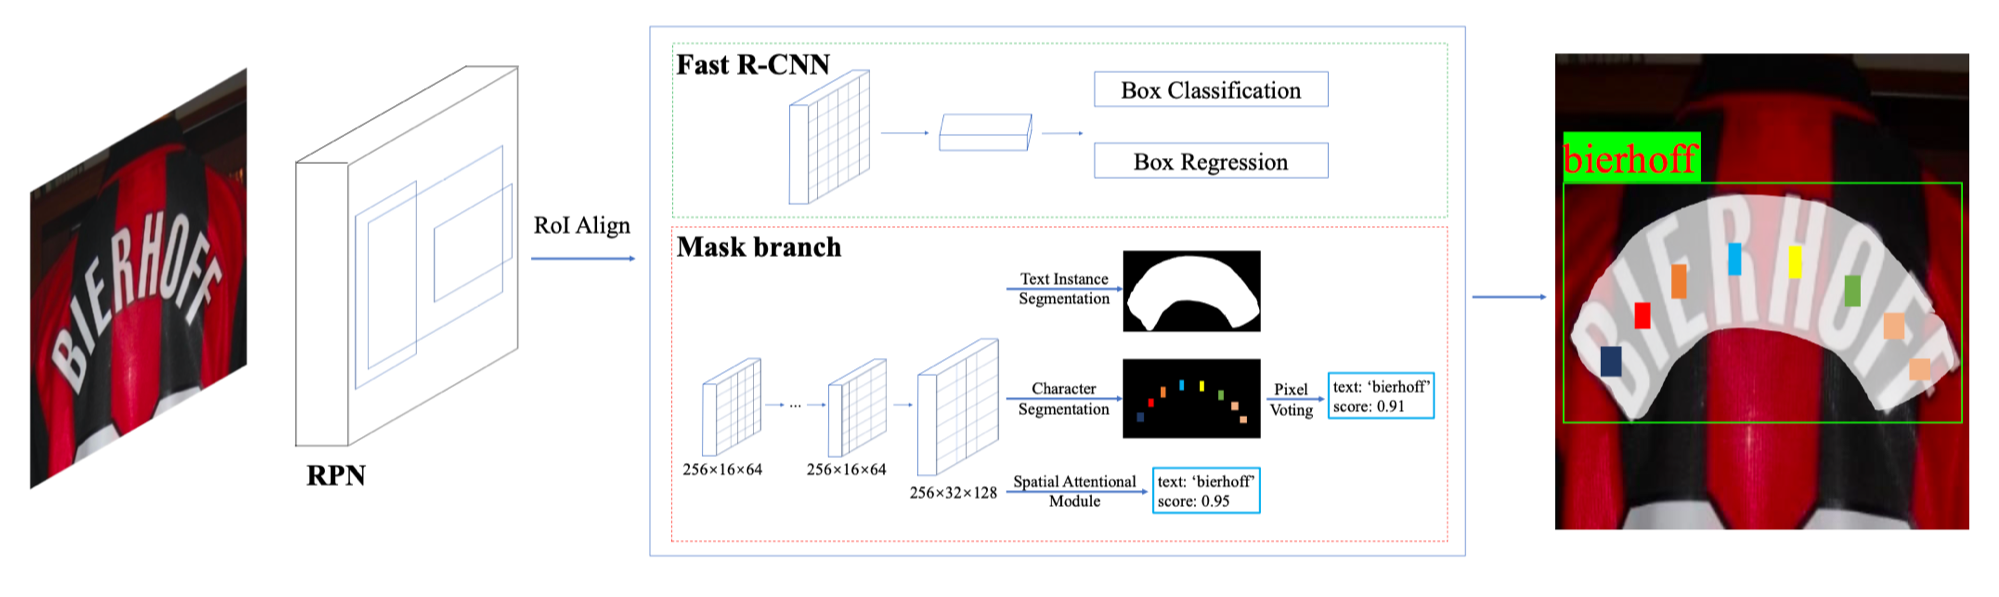
\includegraphics[width=.98\textwidth]{figure/spotting/masktextspotter_v2_framework.png} 
    \caption{MaskTextSpotter\_v2框架图。} 
    \label{masktextspotter_v2_framework} 
\end{figure}

\begin{figure}[htb]
    \centering
    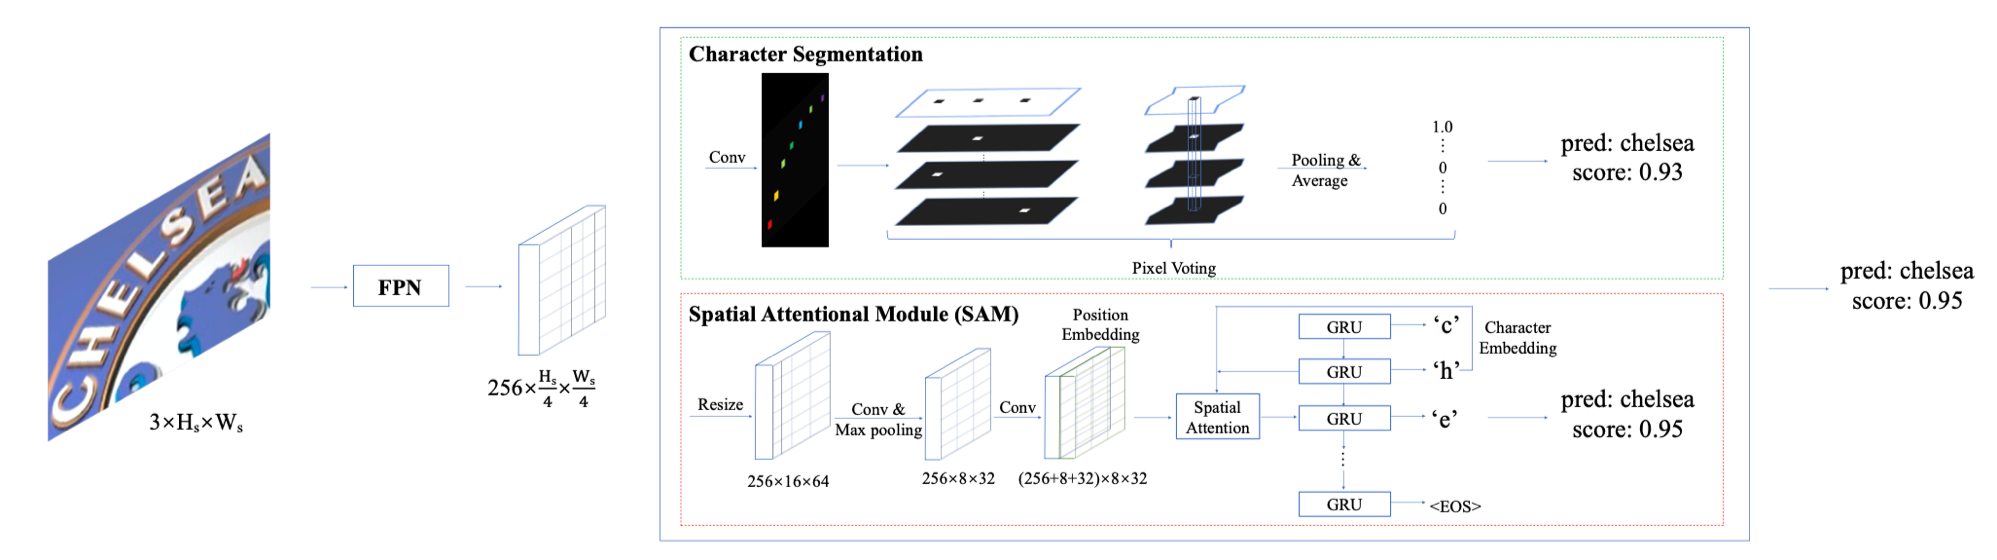
\includegraphics[width=.98\textwidth]{figure/spotting/masktextspotter_v2_recog.png} 
    \caption{MaskTextSpotter\_v2识别分支结构图。} 
    \label{masktextspotter_v2_recog} 
\end{figure}

\subsubsection{MaskTextSpotter\_v2实验细节}
MaskTextSpotter的训练过程分为两部分:合成数据集预训练和真实数据集微调阶段。
合成数据集使用的是SynthText\cite{gupta2016synthetic},batch size为8,输入图像
以短边为800,保持长宽比,学习率从0.001开始,第100k,200k次下降0.1,训练270k步。
在真实数据微调阶段,batch size为8,采用多尺度训练的策略,短边分为(600,800,1000,1200,1400)三个尺度进行训练,
使用的数据集有SynthText, ICDAR2013, ICDAR2015, TotalText以及来自\cite{zhong2016deeptext}的1162张图像。
学习率从0.001开始,第100k下降0.1,训练150k步。

\subsection{TextDragon}
虽然MaskTextSpotter能够进行任意形状文本端到端的识别,但是数据集字符级别的标注的要求使得网络的训练比较昂贵。TextDragon
意在只使用单词级别的标注来设计任意形状文本端到端识别系统。
\subsubsection{TextDragon网络结构}
TextDragon对任意形状文本的表示方式主要来自于文字检测方法TextSnake\cite{long2018textsnake},也就是将任意形状
的文本表示为一系列的带方向正方形。然后从属于同一文本实例的带方向正方形中聚合,采样一个子集形成文本区域。基于该子集的带方向正方形,
则有:
1)从这些带方向正方形中提取文字边界点来表示检测结果,2)对每个正方形区域的特征进行字符分类,通过CTC解码成文本字符串。
TextDragon的网络结构如图\ref{textdragon_framework}所示。

具体地,文字的表示方法如图\ref{textdragon_representation}所示。文本实例由文本的中心线、正方形边长以及正方形旋转方向构成。
在测试阶段,推理过程如下:1)通过文本中心线来获取每个文本实例大致区域;2)在每个文本实例的中心线上获得所有的预测的带方向正方形,
并保留这些IOU大于0.5,旋转角度差小于45度的正方形区域;3)根据其位置将这些保留的正方形进行排序,形成表示该文本区域的正方形子集。
4)最终通过RoISlide从这些矫正后的文本区域中获取特征,进行字符串识别,而文本边界由正方形子集形成的边界点构成。
\begin{figure}[htb]
    \centering
    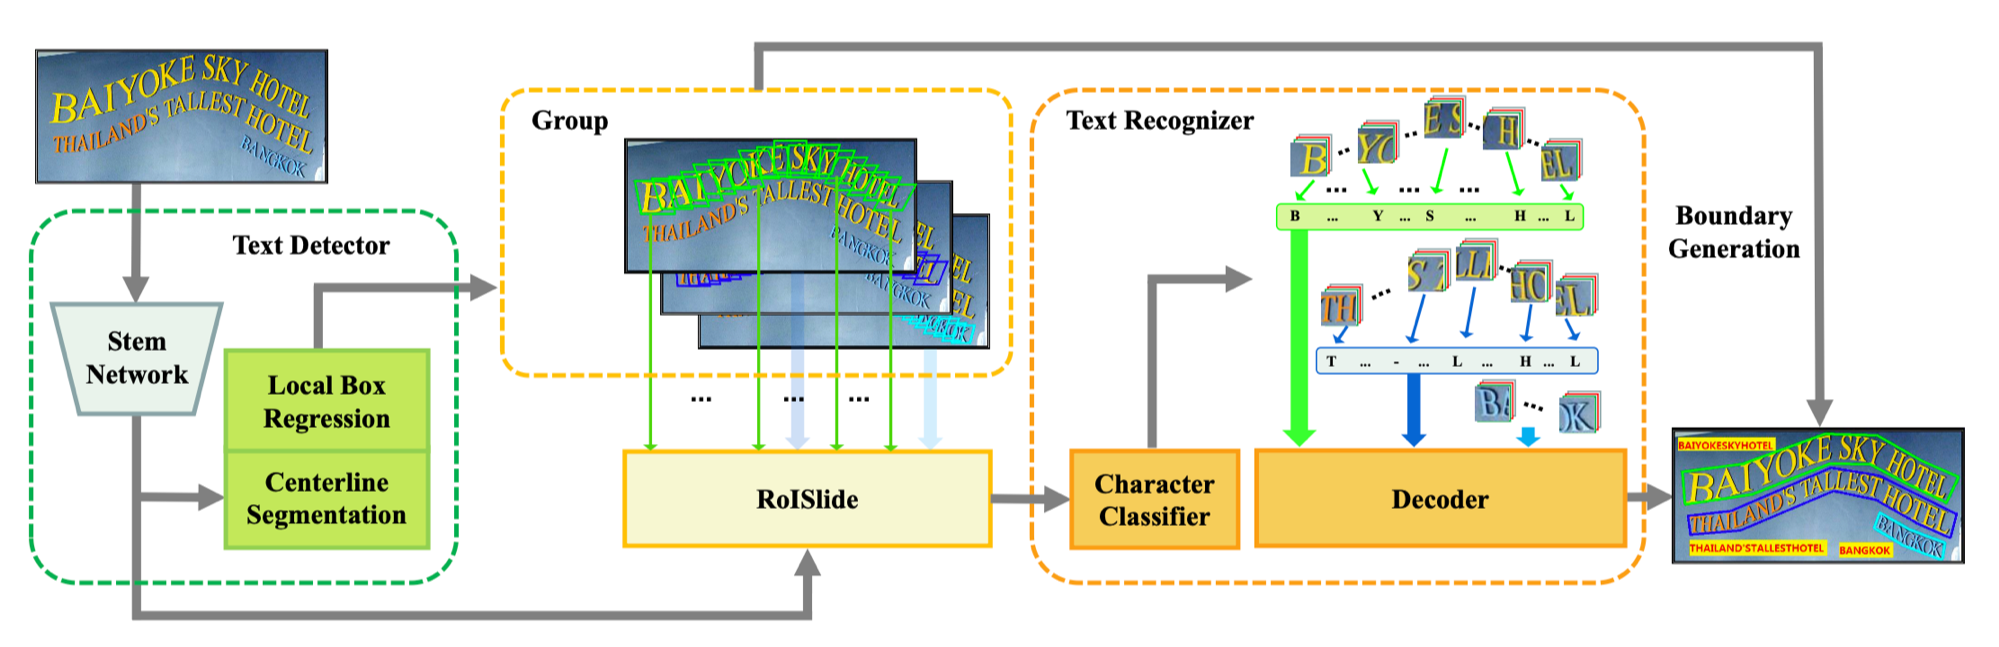
\includegraphics[width=.98\textwidth]{figure/spotting/textdragon_framework.png} 
    \caption{TextDragon框架图。} 
    \label{textdragon_framework} 
\end{figure}

\begin{figure}[htb]
    \centering
    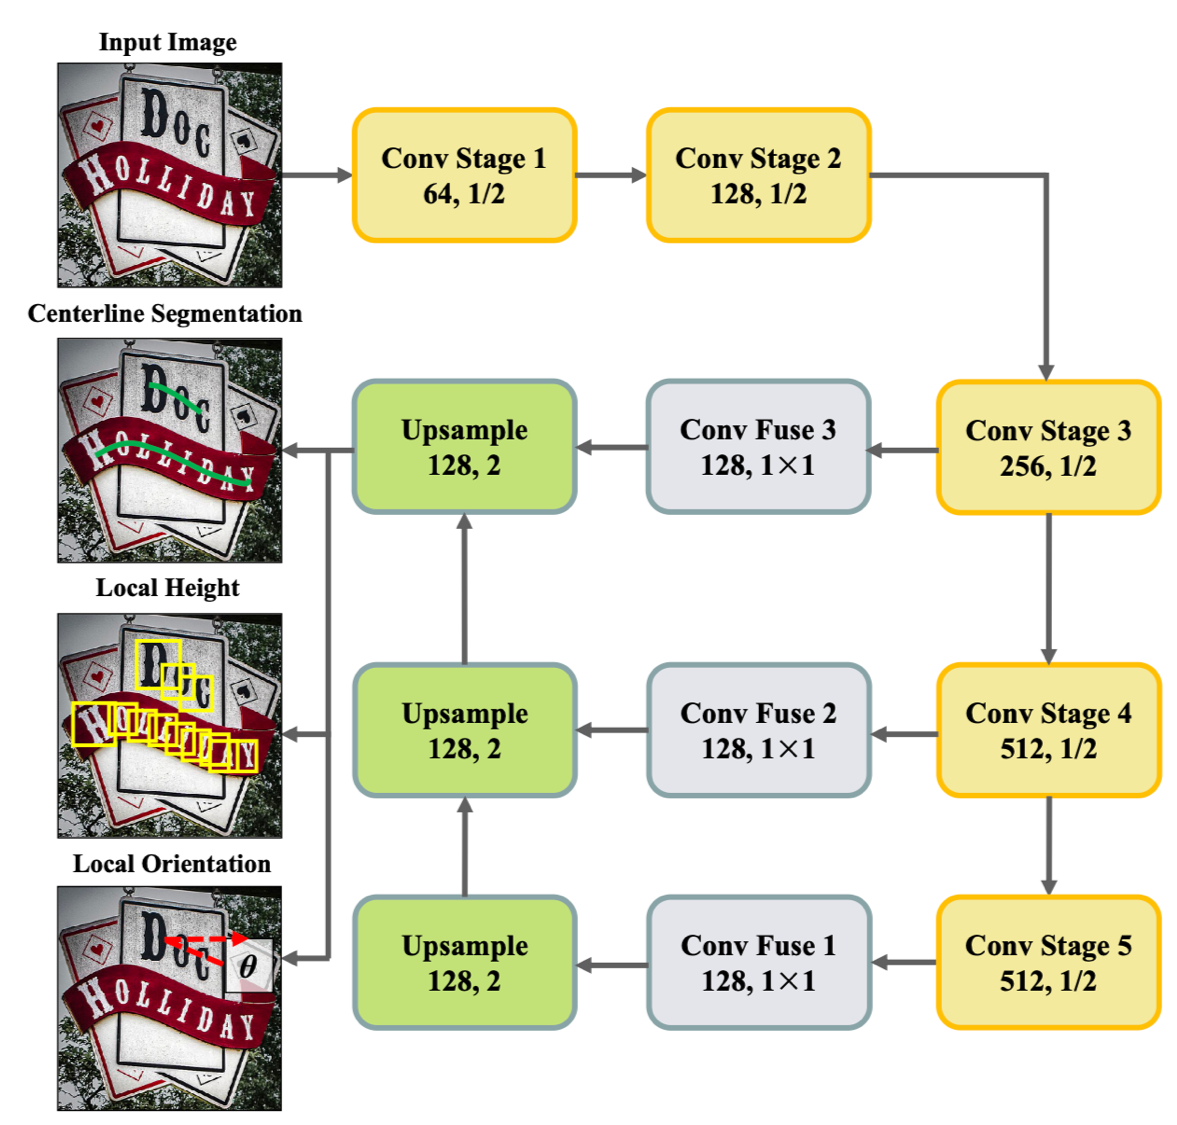
\includegraphics[width=.7\textwidth]{figure/spotting/textdragon_representation.png} 
    \caption{TextDragon文本实例表示方法。} 
    \label{textdragon_representation} 
\end{figure}

\subsubsection{TextDragon实验细节}
TextDragon的训练过程分为两部分:合成数据集预训练和真实数据集微调阶段。
合成数据集使用的是SynthText,输入图像大小为512*512,学习率为0.01,训练600k步。
在真实数据微调阶段,输入图像大小为512*512,数据集为相对应数据集的训练集,学习率为0.001,训练120k步。

\subsection{CharNet}
CharNet与TextDragon一样是在任意形状文本端到端识别算法只有MaskTextSpotter的背景下出现的方法。他的主要出发点是:当前端到端识别的方法中,
都是two stage的(这里two stage是指检测网络得到检测结果,再根据检测结果利用RoI操作获取特征进行识别),作者认为two stage中RoI提取很难提取
准确(主要是检测存在误差),并且two stage过程繁琐,不便使用。因此,作者想设计一个single stage的网络,同时输出文本实例的检测和识别结果。
\subsubsection{CharNet网络结构}
CharNet在核心问题上和MaskTextSpotter一致,都是通过字符级别的分割解决任意形状文本的识别问题。MaskTextSpotter是在RoI内进行分割,而CharNet是在
全图进行字符级别的分割。那么,CharNet就剩下最后一个需要解决的问题:如何将分割出的字符group成为一个文本区域?
如CharNet网络结构图\ref{charnet_framework}所示,其Detection Branch的作用便是预测一些信息来将分割出的字符聚合成字符串。
对于多方向文本,其Detection Branch的表示方法为EAST\cite{zhou2017east}的表示方式,利用预测的四边形框的IoU聚合每个字符为字符串。
对于曲形文本,其Detection Branch的表示方法为TextField\cite{xu2019textfield}的表示方法。
\begin{figure}[htb]
    \centering
    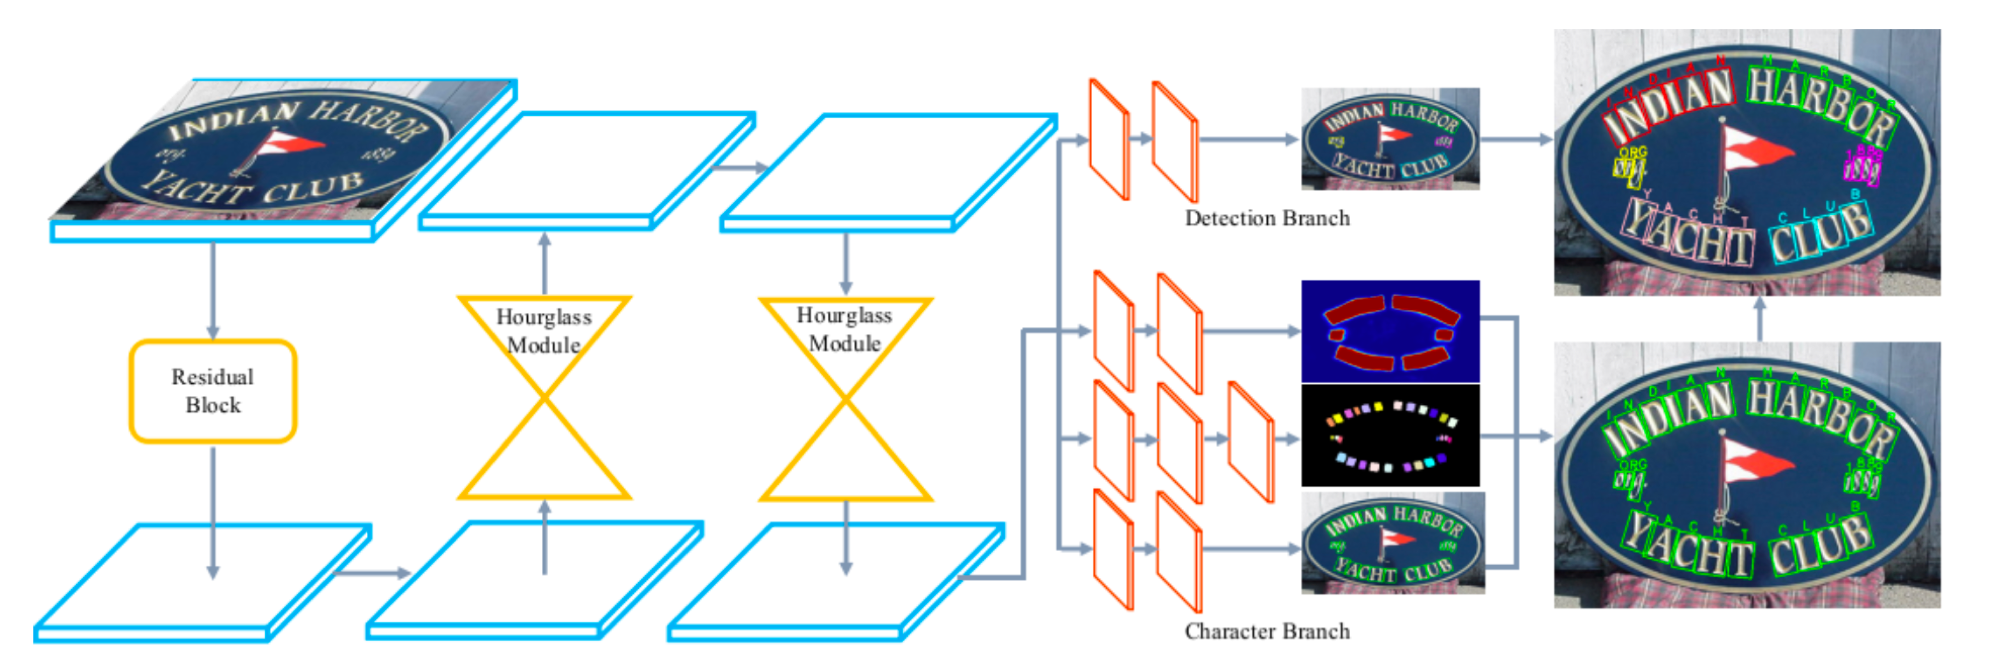
\includegraphics[width=.98\textwidth]{figure/spotting/charnet_framework.png} 
    \caption{CharNet框架图。} 
    \label{charnet_framework} 
\end{figure}

\subsubsection{CharNet实验细节}
CharNet的训练过程分为两部分:合成数据集预训练和真实数据集微调阶段。
合成数据集使用的是SynthText,batch size为32,学习率为0.0002,数据集迭代5 epochs。
在真实数据微调阶段,数据集为相对应数据集的训练集,学习率为0.002,分三步进行迭代训练,三步训练回合分别为100,400,800epochs。
这里每步迭代训练是指:利用先前的模型获得训练集的字符级别标注(检测框),过滤出正确的字符级别标注来训练模型,迭代n(100,400或800)个epochs。

\subsection{MaskRoI}
MaskRoI与CharNet以及TextDragon是同时期文章,该方法不需要字符级别的标注,同时不需要将任意形状文本矫正为水平文本进行识别。
\subsubsection{MaskRoI网络结构}
如图\ref{maskroi_framework}所示,MaskRoI和MaskTextSpotter一样,也是基于MaskRCNN框架进行改进的。识别分支采用基于attention的序列识别方案。
为了解决任意形状文本的RoI容易采样到背景或者相邻文本特征的问题,在进行序列识别之前,进行了特征过滤操作。该操作就是将文本实例分割图和RoI的特征进行相乘。

\begin{figure}[htb]
    \centering
    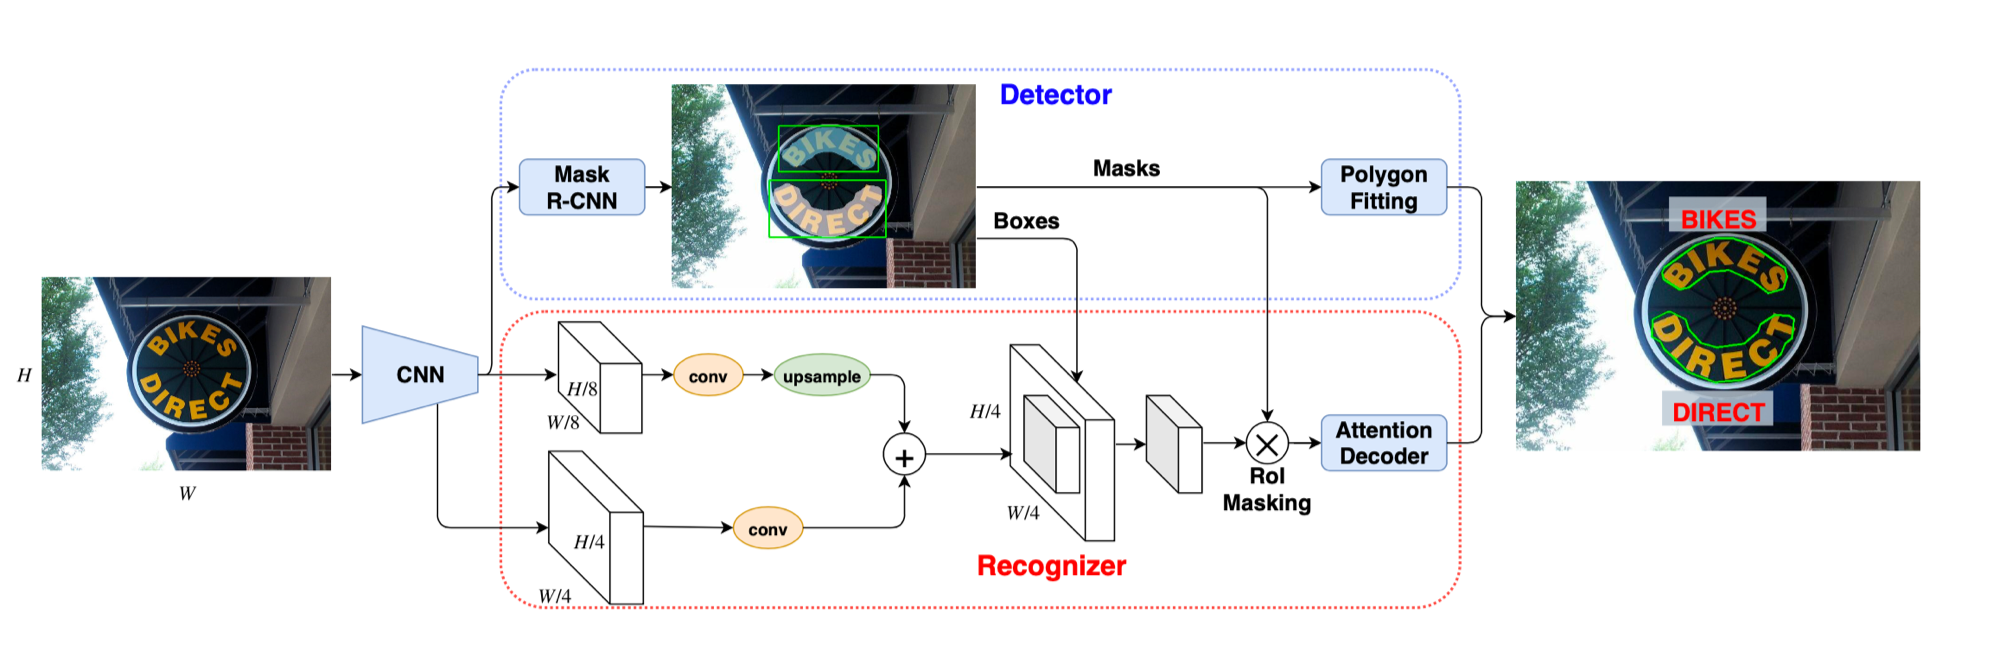
\includegraphics[width=.98\textwidth]{figure/spotting/maskroi_framework.png} 
    \caption{MaskRoI框架图。} 
    \label{maskroi_framework} 
\end{figure}

\subsubsection{MaskRoI实验细节}
MaskRoI采用一步训练的方式,数据集包括SynthText,ICDAR2015,COCOText,ICDAR-MLT,TotalText以及网络收集的通过Google OCR Api标注的30k张图像。
采用多尺度训练的策略,短边为480到800之间。

\subsection{Boundary}

\subsection{TextPerceptron}
TextPerceptron的主体思路也是文本实例边界点检测+TPS+序列识别。和Boundary不同之处在于文本边检点检测过程,具体地说,是通过文本实例的几何属性和后处理得到
边界点。
\subsubsection{TextPerceptron网络结构}
TextPerceptron的网络结构如图\ref{textperceptron_framework}所示。边界点的检测是基于分割的方法,预测的文本实例的几何属性包括:1)文本上下边界;2)文本实例的开端;
3)文本实例的结尾;4)文本实例的中间区域;5)开端以及结尾处的角点回归;6)文本中心区域的边界点回归。其中5)和6)的标签定义如图\ref{textperceptron_label}所示。
\begin{figure}[htb]
    \centering
    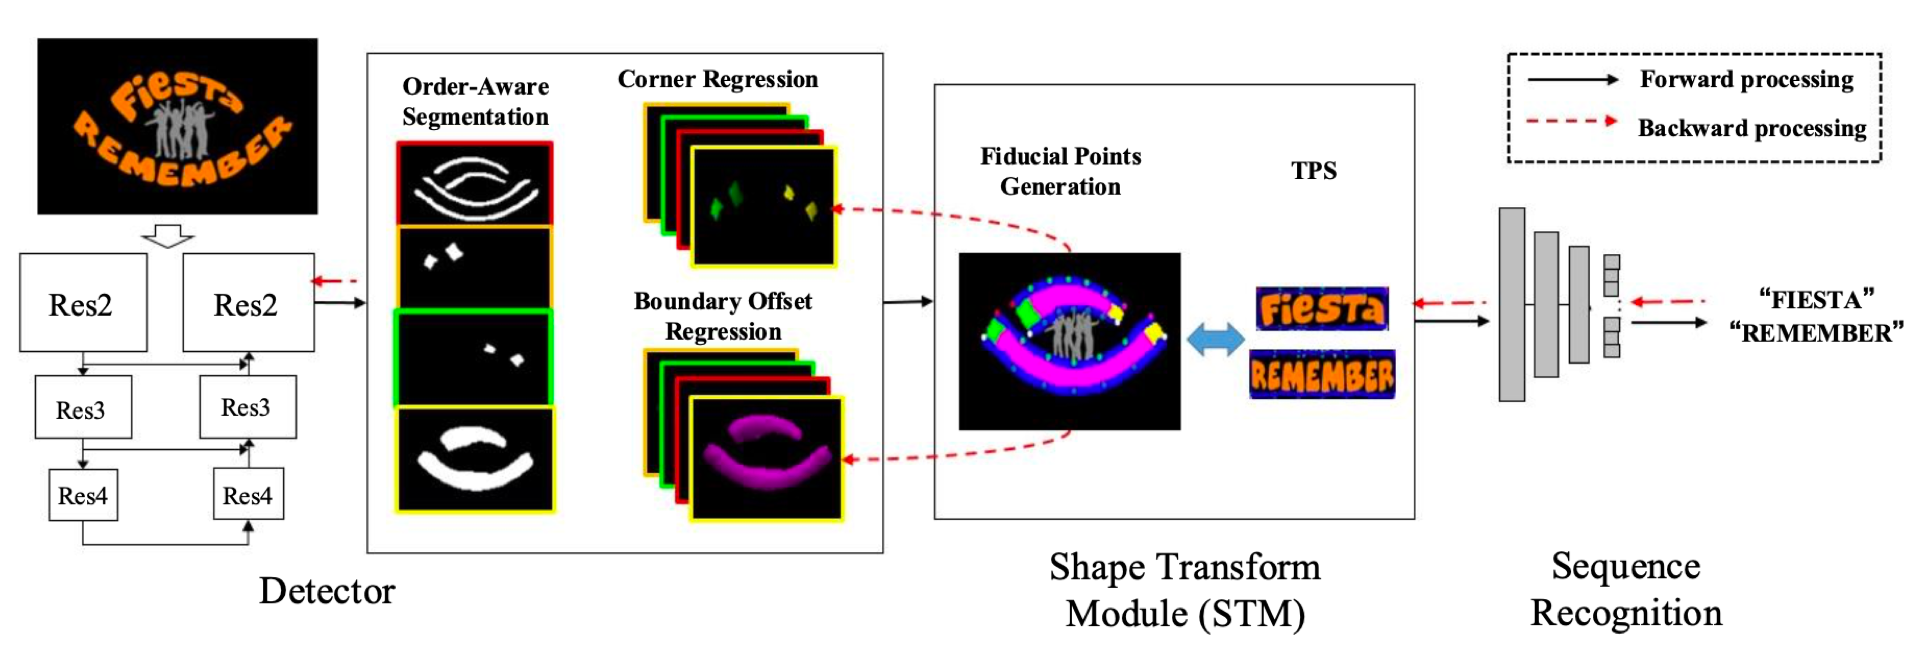
\includegraphics[width=.98\textwidth]{figure/spotting/textperceptron_framework.png} 
    \caption{TextPerceptron框架图。} 
    \label{textperceptron_framework} 
\end{figure}

\begin{figure}[htb]
    \centering
    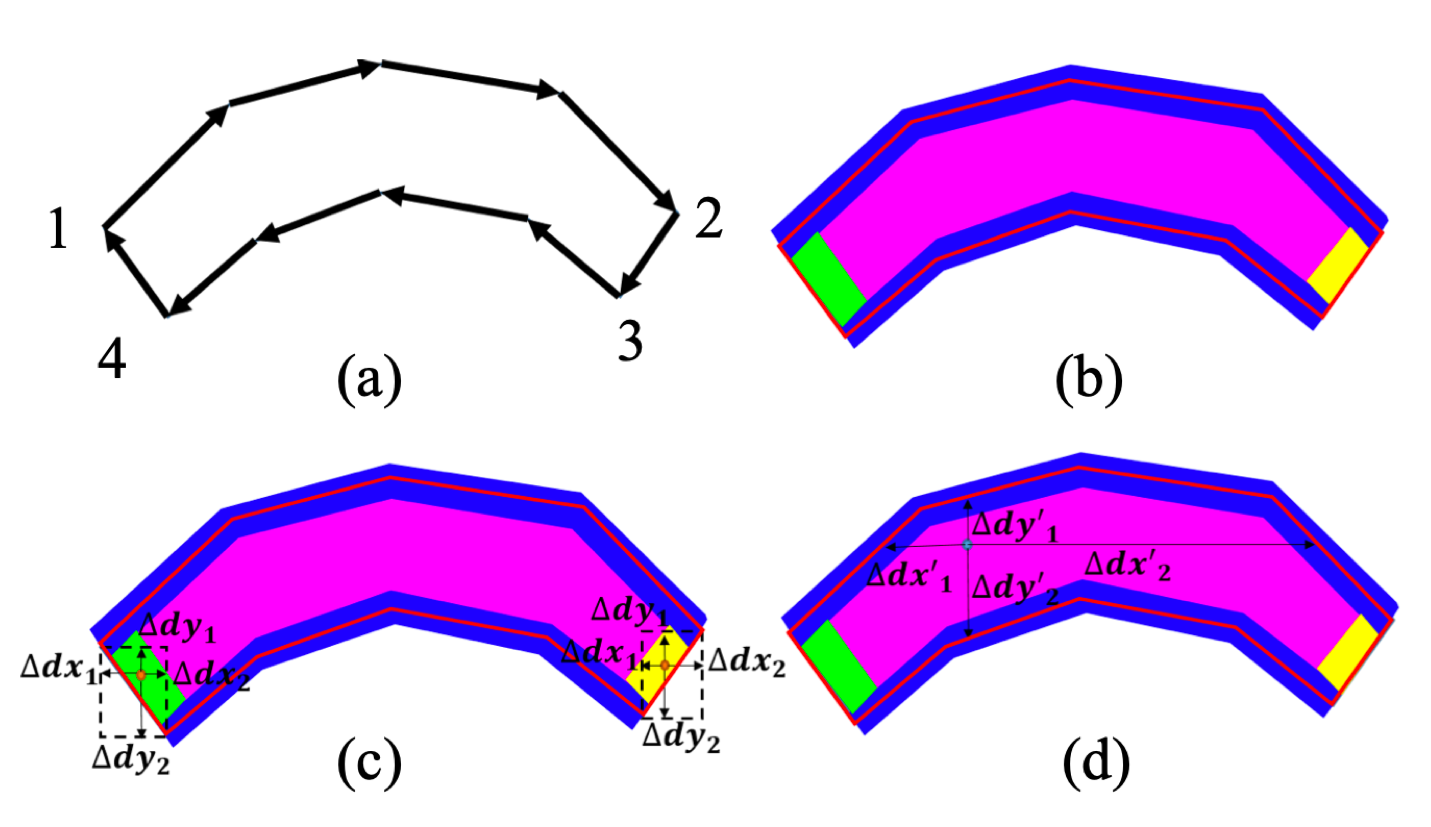
\includegraphics[width=.8\textwidth]{figure/spotting/textperceptron_label.png} 
    \caption{TextPerceptron 角点和边界点回归的定义。} 
    \label{textperceptron_label} 
\end{figure}

\subsubsection{TextPerceptron边界点获取过程}
根据预测的文本实例的几何属性,后处理得到边界点的过程如下:
1)根据中心区域和开端以及结尾的匹配程度可以获得开端、结尾匹配对,上下边界可以用于区分相邻的文本实例;
2)在开端、结尾分割图处获取文本实例的4个角点;
3)如图\ref{textperceptron_process}所示,获得较长边的角点对的中心点,作垂线,获得该点对所处边界的交点作为一个边界点,以此类推,获得所有边界点。
\begin{figure}[htb]
    \centering
    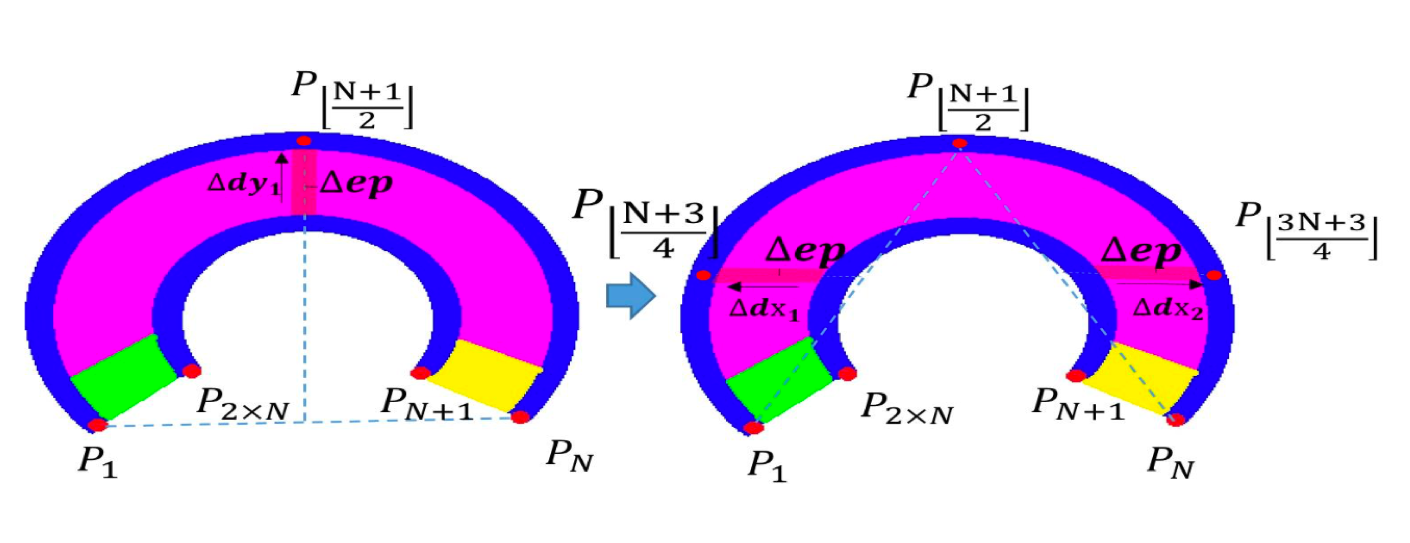
\includegraphics[width=.8\textwidth]{figure/spotting/textperceptron_process.png} 
    \caption{TextPerceptron后处理过程。} 
    \label{textperceptron_process} 
\end{figure}

\subsubsection{TextPerceptron实验细节}
TextPerceptron分为3个阶段,1)训练检测分支,在SynthText上以学习率0.002训练5 epochs;2)训练识别分支,在SynthText上以学习率0.002训练5 epochs;
3)检测识别联合训练,在各自训练集上以学习率0.001训练80 epochs,每20 epochs学习率乘以0.1。


\subsection{ABCNet}
ABCNet的主体思路也是文本实例边界点检测+TPS+序列识别。边界点的检测采样回归的方法,和Boundary不同的是,检测部分采用anchor-free的方法。论文的框架主要基于FCOS\cite{tian2019fcos}上进行改进。
\subsubsection{ABCNet网络结构}
ABCNet采用贝塞尔曲线来表示文本实例的边界,贝塞尔曲线描述效果如图\ref{abcnet_basier}所示。网络框架如图\ref{abcnet_framework}所示,FCOS采用密集预测的方式。从代码中可以看出,检测部分的预测信息包括:
1)每个bbox的得分;2)中心区域预测;3)bbox回归;4)贝塞尔曲线控制点预测。
获得贝塞尔曲线后,
\begin{figure}[htb]
    \centering
    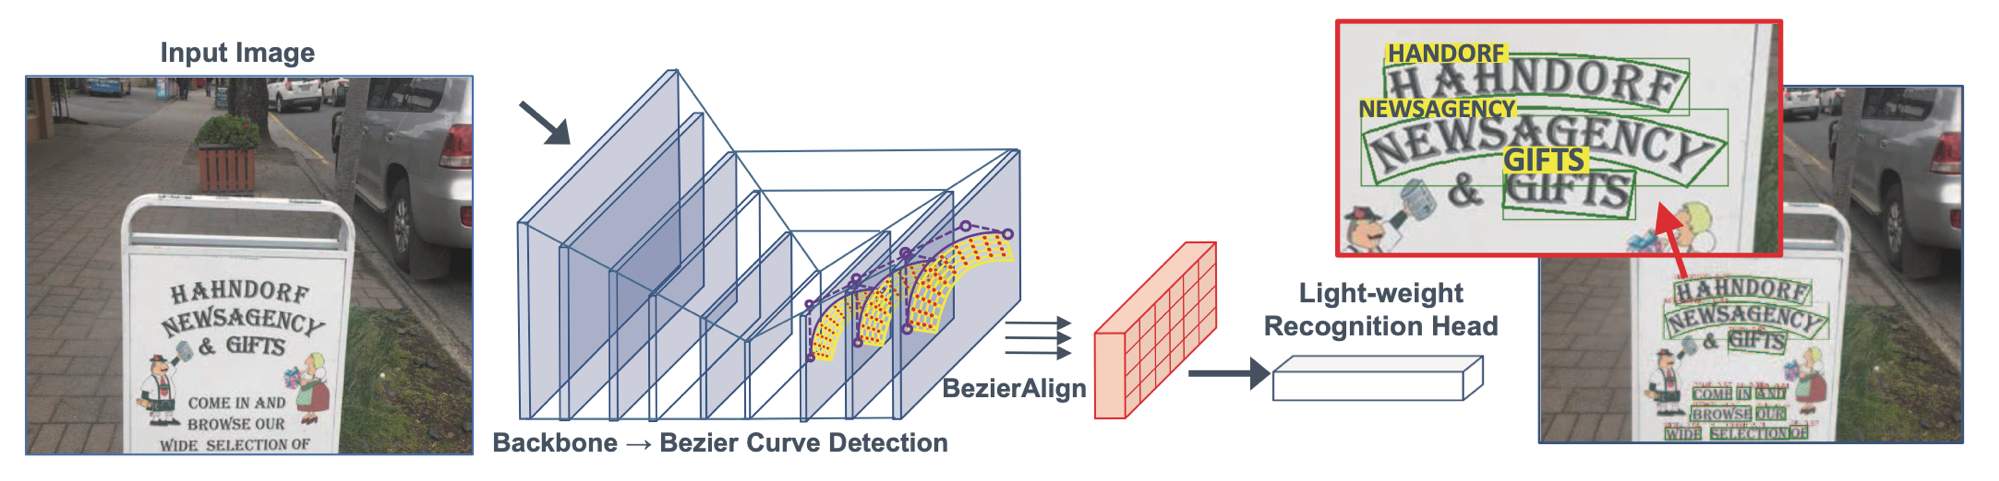
\includegraphics[width=.98\textwidth]{figure/spotting/abcnet_framework.png} 
    \caption{ABCNet框架图。} 
    \label{abcnet_framework} 
\end{figure}

\begin{figure}[htb]
    \centering
    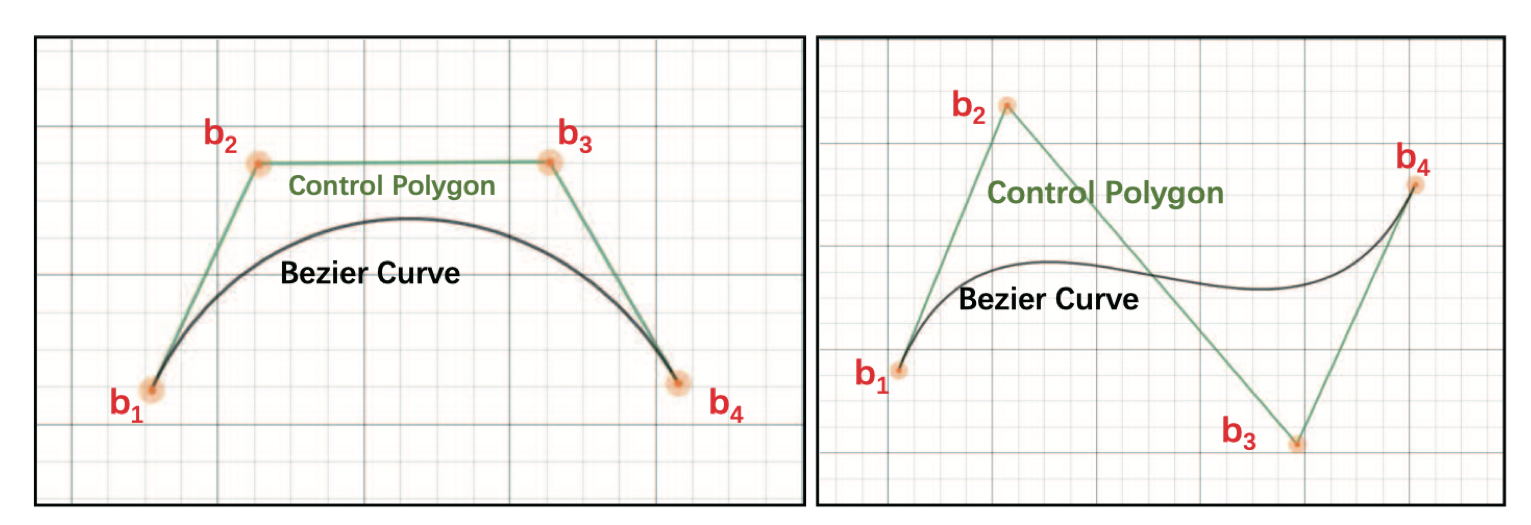
\includegraphics[width=.98\textwidth]{figure/spotting/abcnet_basier.png} 
    \caption{贝塞尔曲线。} 
    \label{abcnet_basier} 
\end{figure}

贝塞尔曲线获得的边界如图\ref{abcnet_sample}所示。
\begin{figure}[htb]
    \centering
    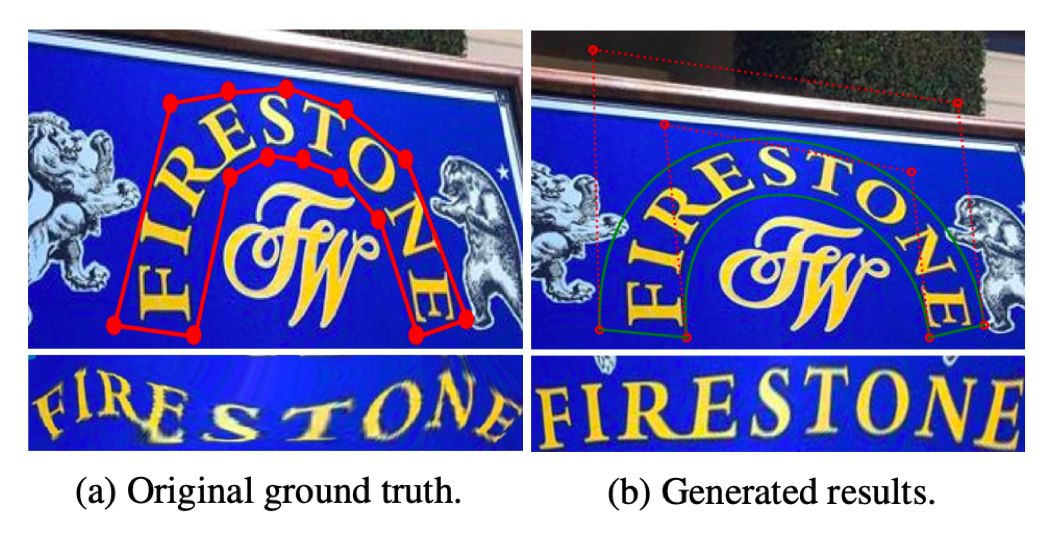
\includegraphics[width=.98\textwidth]{figure/spotting/abcnet_sample.png} 
    \caption{贝塞尔曲线。} 
    \label{abcnet_sample} 
\end{figure}

\subsubsection{ABCNet实验细节}
TextPerceptron分为2个阶段:1)合成的150k合成数据集,15k的COCOText,7k的ICDAR-MLT预训练;2)相应的训练集训练。

\section{任意形状文本端到端识别方法的总结}

% %# -*- coding: utf-8-unix -*-
%%==================================================
\chapter{这是什么?}

这是$\mathbb{ Q}$-book \LaTeX 书籍模板,当前版本为 \version 。

这份模板主要基于上海交大的学位论文模板
\footnote{\url{https://github.com/sjtug/SJTUThesis}}修改得到
,结合少量个人审美喜好,重新定制了定义、定理等环境。由于这个模板本是用于一项书籍翻译计划,因此其中的一些环境,例如“观察”、“规则”、“关键点”等,读者可能用不到,可以根据自己的需求适当修改。

你也可以通过邮箱\texttt{jey74165@163.com}给我发邮件反映遇到的问题。不过作者水平有限,或许有些问题也无法解答,还请见谅。

\section{文档说明}

\subsection{准备工作}

要想灵活使用、魔改这个模板来撰写自己的书籍,需要对\emph{TeX系统}有一定的了解,也需要掌握基本的\emph{TeX技能}。

\begin{itemize}[noitemsep,topsep=0pt,parsep=0pt,partopsep=0pt]
	\item {\TeX}系统:所使用的{\TeX}系统要支持 \XeTeX 引擎,且带有ctex 2.x宏包。一般来说,只要安装了的\emph{完整}TeXLive或MacTeX发行版就不会出现问题。
	\item TeX技能:尽管提供了对模板的必要说明,但这并不是一份“ \LaTeX 入门文档”。用户应当有一定的\LaTeX 使用经验。
\end{itemize}

\subsection{字体与选项}

$\mathbb{ Q }$-book暂不提供可选项,直接用命令\verb|\documentclass{qbook}|载入即可。如有需要,用户可以根据自己的需求进行相关的添加或修改。

本模板所使用的字体仅为宋体,{\kaishu{楷体}}和{\heiti{黑体}}等自带字体,用户不会在字体问题上折腾太多精力。

\subsection{编译方式}

最简单的办法是直接双击模板文件夹中的compile.bat文件,在命令行模式下编译;当然使用你配置好的Tex编辑器也是可以的。编译失败时,可以尝试手动逐次编译,定位故障。
\begin{lstlisting}[basicstyle=\small\ttfamily, caption={手动逐次编译}, numbers=none]
xelatex -no-pdf qbook
biber --debug qbook
xelatex qbook
xelatex qbook
\end{lstlisting}

\section{模板文件介绍}

本节介绍$\mathbb{ Q }$-book模板中主要文件和目录的功能。

\subsection{格式控制文件}

格式控制文件控制着书籍的表现形式,包括以下两个文件
\begin{itemize}[noitemsep,topsep=0pt,parsep=0pt,partopsep=0pt]
	\item qbook.cfg
	\item qbook.cls
\end{itemize}
其中,“cfg”和“cls”为文件格式。

\subsection{主文件}

主文件qbook.tex的作用就是将你分散在多个文件中的章节重新“拼合”成一本完整的书。
当我们用\LaTeX 写书时,肯定不希望一直在同一页面码字,那样会显得非常臃肿,而且不便于以后的修改和查找。所以在使用本模板的时候,你的章节内容和素材会被“拆散”为各个部分,例如前言、概览、各章节及参考文献等。
在qbook.tex中通过\verb|\include{xxx}|命令将各个部分包含进来,从而形成一本结构完整的书籍。

\subsection{各部分源文件}

被“拆散”的各个部分的源文件存放于tex文件夹中,是论文的主体,以“章”为单位划分,其中包括:

\begin{itemize}[noitemsep,topsep=0pt,parsep=0pt,partopsep=0pt]
	\item cover.tex——用于绘制封面。
	\item preface.tex——前言。
	\item overview.tex——概览。
	\item chapter(xxx).tex——各章主体内容。
	\item 参考文献列表由bibtex插入,不作为一个单独的文件。
\end{itemize}

\subsection{图片存放}

figure文件夹放置了需要插入文档中的图片文件(支持PNG/JPG/PDF/EPS格式的图片)。
在qbook.cls中已经使用\verb|\graphicspath|命令定义了图片存储的顶层目录,所以在插入图片时,图片路径的顶层目录名“figure”可省略。

\subsection{参考文献数据库}

目前参考文件数据库目录只存放一个参考文件数据库qbook.bib。
关于参考文献引用,可参考第\ref{chap2}章中的例子。

% %# -*- coding: utf-8-unix -*-
%%==================================================

\chapter{写作示例}
\label{chap2}

\section{列表环境}

\subsection{无序列表}

以下是一个无序列表的例子,列表的每个条目单独分段。

\begin{itemize}
	\item 这是一个无序列表。
	\item 这是一个无序列表。
	\item 这是一个无序列表。
\end{itemize}

使用\verb+itemize*+环境可以创建行内无序列表。
\begin{itemize*}
	\item 这是一个无序列表
	\item 这是一个无序列表
	\item 这是一个无序列表
\end{itemize*}
行内无序列表条目不单独分段,所有内容直接插入在原文的段落中。

\subsection{有序列表}

使用环境\verb+enumerate+和\verb+enumerate*+创建有序列表,
使用方法无序列表类似。
\begin{enumerate}
	\item 这是一个有序列表。
	\item 这是一个有序列表。
	\item 这是一个有序列表。
\end{enumerate}

使用\verb+enumerate*+环境可以创建行内有序列表。
\begin{enumerate*}
	\item 这是一个默认有序列表
	\item 这是一个默认有序列表
	\item 这是一个默认有序列表
\end{enumerate*}
行内有序列表条目不单独分段,所有内容直接插入在原文的段落中。

\subsection{描述列表}
使用环境\verb+description+可创建带有主题词的列表,条目语法是\verb+\item[主题] 内容+。
\begin{description}
	\item[主题一] 详细内容
	\item[主题二] 详细内容
	\item[主题三] 详细内容 \ldots
\end{description}

\section{数学排版}

\subsection{公式排版}

这里有举一个长公式排版的例子,来自\href{http://www.tex.ac.uk/tex-archive/info/math/voss/mathmode/Mathmode.pdf}{《Math mode》}:

\begin {multline}
\frac {1}{2}\Delta (f_{ij}f^{ij})=
2\left (\sum _{i<j}\chi _{ij}(\sigma _{i}-
\sigma _{j}) ^{2}+ f^{ij}\nabla _{j}\nabla _{i}(\Delta f)+\right .\\
\left .+\nabla _{k}f_{ij}\nabla ^{k}f^{ij}+
f^{ij}f^{k}\left [2\nabla _{i}R_{jk}-
\nabla _{k}R_{ij}\right ]\vphantom {\sum _{i<j}}\right )
\end{multline}

\subsection{SI单位}

使用\verb+siunitx+宏包可以方便地输入SI单位制单位,例如\verb+\SI{5}{\um}+可以得到\SI{5}{\um}。

\subsection{定理环境}

在这个模板中,定义了如下几个环境
remark(注),mythm(定理),myprop(性质),mydef(定义),example(例)。
amsmath还提供了一个proof(证明)的环境。
我们举例说明它们的用法。

注环境
\begin{remark}
	存在事先给定的一系列基本操作,并且这些基本操作永远不会改变。
\end{remark}
\begin{remark}
	每个操作都可逆。
	\label{o1.2}
\end{remark}
\begin{remark}
	每一个操作都是确定性的。
\end{remark}
\begin{remark}
	各个操作可以按任何顺序组合。
\end{remark}

性质环境
\begin{myprop}{}{}
	存在一些预先定义的永不发生改变的作用(action)。
\end{myprop}

\begin{myprop}{}{}
	每一个作用都可逆。
\end{myprop}

\begin{myprop}{}{}
	每个作用都是确定性的。
\end{myprop}

\begin{myprop}{}{}
	任意的一系列连续的作用仍然是一个作用。
\end{myprop}

例子环境
\begin{example}
	天地玄黄,宇宙洪荒。
	\soln
	
	日月盈仄,辰宿列张。
\end{example}

定义环境
\begin{mydef}{域}{1}
	设$S$为一个非空集合,其上有“加法”(记作$+$)与“乘法”(记作$\cdot$)两种代数运算. 若满足以下条件,则称$(S,+,\cdot)$构成一个域(field).
	\begin{itemize}
		\item[(1)] $(S,+)$构成一个交换群.
		\item[(2)] 若记$S^{*}=S-\{0\}$,其中$0$为群$(S,+)$中的单位元,则$(S^{*},\cdot)$也构成一个交换群.
		\item[(3)] 乘法对加法有分配律:$a ( b + c ) = a b + a c$.
	\end{itemize}
\end{mydef}

关键点环境
\begin{keypoint}
	伽罗瓦理论在分析从有理数域$\mathbb{ Q }$扩张到新的域的运算或操作时很有用。我们的大问题可以用伽罗瓦理论来回答,数学中其他的一些历史问题也同样可以用伽罗瓦理论来解答。
\end{keypoint}

定理环境
\begin{mythm}{望远镜公式}{2}
	$\left[\mathbb{Q}(a, b) : \mathbb{Q}\right]=\left[\mathbb{Q}(a, b) : \mathbb{Q}(a)\right]\left[\mathbb{Q}(a) : \mathbb{Q}\right] $
\end{mythm}

\begin{proof}
	
	\rthm{thm:2}告诉我们,对任意$s\in S$,均有$\lvert Orb(s)\rvert \cdot \lvert Stab(s)\rvert=\lvert G\rvert=p$. 于是$\lvert Orb(s)\rvert $整除$p$,这里$p$是一个素数。从而$\lvert Orb(s)\rvert $等于1或$p$,也就是说,\textbf{所有轨道的大小要么为1,要么为$p$}. 于是整个集合$S$就被划分为两部分,一部分是大小为1的轨道,另一部分是大小为$p$的轨道,如图9.4所示。
	
	假设大小为1的轨道有$m$个,大小为$p$的轨道有$n$个,则有
 \begin{equation}
		m+p\cdot n=\lvert S\rvert 
 \end{equation}
	注意到\rdef{def:1},\textbf{那些$\lvert Orb(s)\rvert =1$的元素$s$即为稳定元},这就表明有$m$个稳定元。从上式立刻看出$\lvert S \rvert \equiv  m\; (\bmod\; p)$.	
\end{proof}

\section{表格}

这一节给出的是一些表格的例子,如表\ref{tab1}所示。

\begin{table}[!hpb]
	\centering
	\bicaption[指向一个表格的表目录索引]
	{一个颇为标准的三线表格\footnotemark[1]}
	{A Table}
	\label{tab1}
	\begin{tabular}{@{}llr@{}} \toprule
		\multicolumn{2}{c}{Item} \\ \cmidrule(r){1-2}
		Animal & Description & Price (\$)\\ \midrule
		Gnat & per gram & 13.65 \\
		& each & 0.01 \\
		Gnu & stuffed & 92.50 \\
		Emu & stuffed & 33.33 \\
		Armadillo & frozen & 8.99 \\ \bottomrule
	\end{tabular}
\end{table}
\footnotetext[1]{这个例子来自\href{http://www.ctan.org/tex-archive/macros/latex/contrib/booktabs/booktabs.pdf}{《Publication quality tables in LATEX》}(booktabs宏包的文档)。这也是一个在表格中使用脚注的例子,请留意与threeparttable实现的效果有何不同。}

下面一个是一个更复杂的表格,用threeparttable实现带有脚注的表格,如表\ref{tab2}。

\begin{table}[!htpb]
	\bicaption[出现在表目录的标题]
	{一个带有脚注的表格的例子}
	{A Table with footnotes}
	\label{tab2}
	\centering
	\begin{threeparttable}[b]
		\begin{tabular}{ccd{4}cccc}
			\toprule
			\multirow{2}{6mm}{total}&\multicolumn{2}{c}{20\tnote{1}} & \multicolumn{2}{c}{40} &  \multicolumn{2}{c}{60}\\
			\cmidrule(lr){2-3}\cmidrule(lr){4-5}\cmidrule(lr){6-7}
			&www & \multicolumn{1}{c}{k} & www & k & www & k \\ % 使用说明符 d 的列会自动进入数学模式,使用 \multicolumn 对文字表头做特殊处理
			\midrule
			&$\underset{(2.12)}{4.22}$ & 120.0140\tnote{2} & 333.15 & 0.0411 & 444.99 & 0.1387 \\
			&168.6123 & 10.86 & 255.37 & 0.0353 & 376.14 & 0.1058 \\
			&6.761    & 0.007 & 235.37 & 0.0267 & 348.66 & 0.1010 \\
			\bottomrule
		\end{tabular}
		\begin{tablenotes}
			\item [1] the first note.% or \item [a]
			\item [2] the second note.% or \item [b]
		\end{tablenotes}
	\end{threeparttable}
\end{table}

\section{插入图片}

\XeTeX 可以很方便地插入PDF、PNG、JPG格式的图片。插入PNG/JPG的例子如\ref{fig1}所示。
这两个水平并列放置的图共享一个“图标题”(table caption),没有各自的小标题。

\begin{figure}[!htp]
\centering

\includegraphics[width=4cm]{example/by-nc.png}
\hspace{1cm}
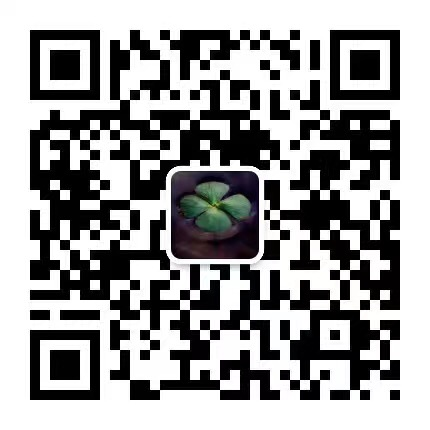
\includegraphics[width=4cm]{example/gzh.jpg}
\bicaption{中文题图}
{English caption}
\label{fig1}
\end{figure}

这里还有插入EPS图像和PDF图像的例子,如图\ref{fig2}和图\ref{fig3}。这里将EPS和PDF图片作为子图插入,每个子图有自己的小标题。子图标题使用subcaption宏包添加。

\begin{figure}[!htp]
\centering
\subcaptionbox{EPS 图像\label{fig2}}[3cm] %标题的长度,超过则会换行,如下一个小图。
{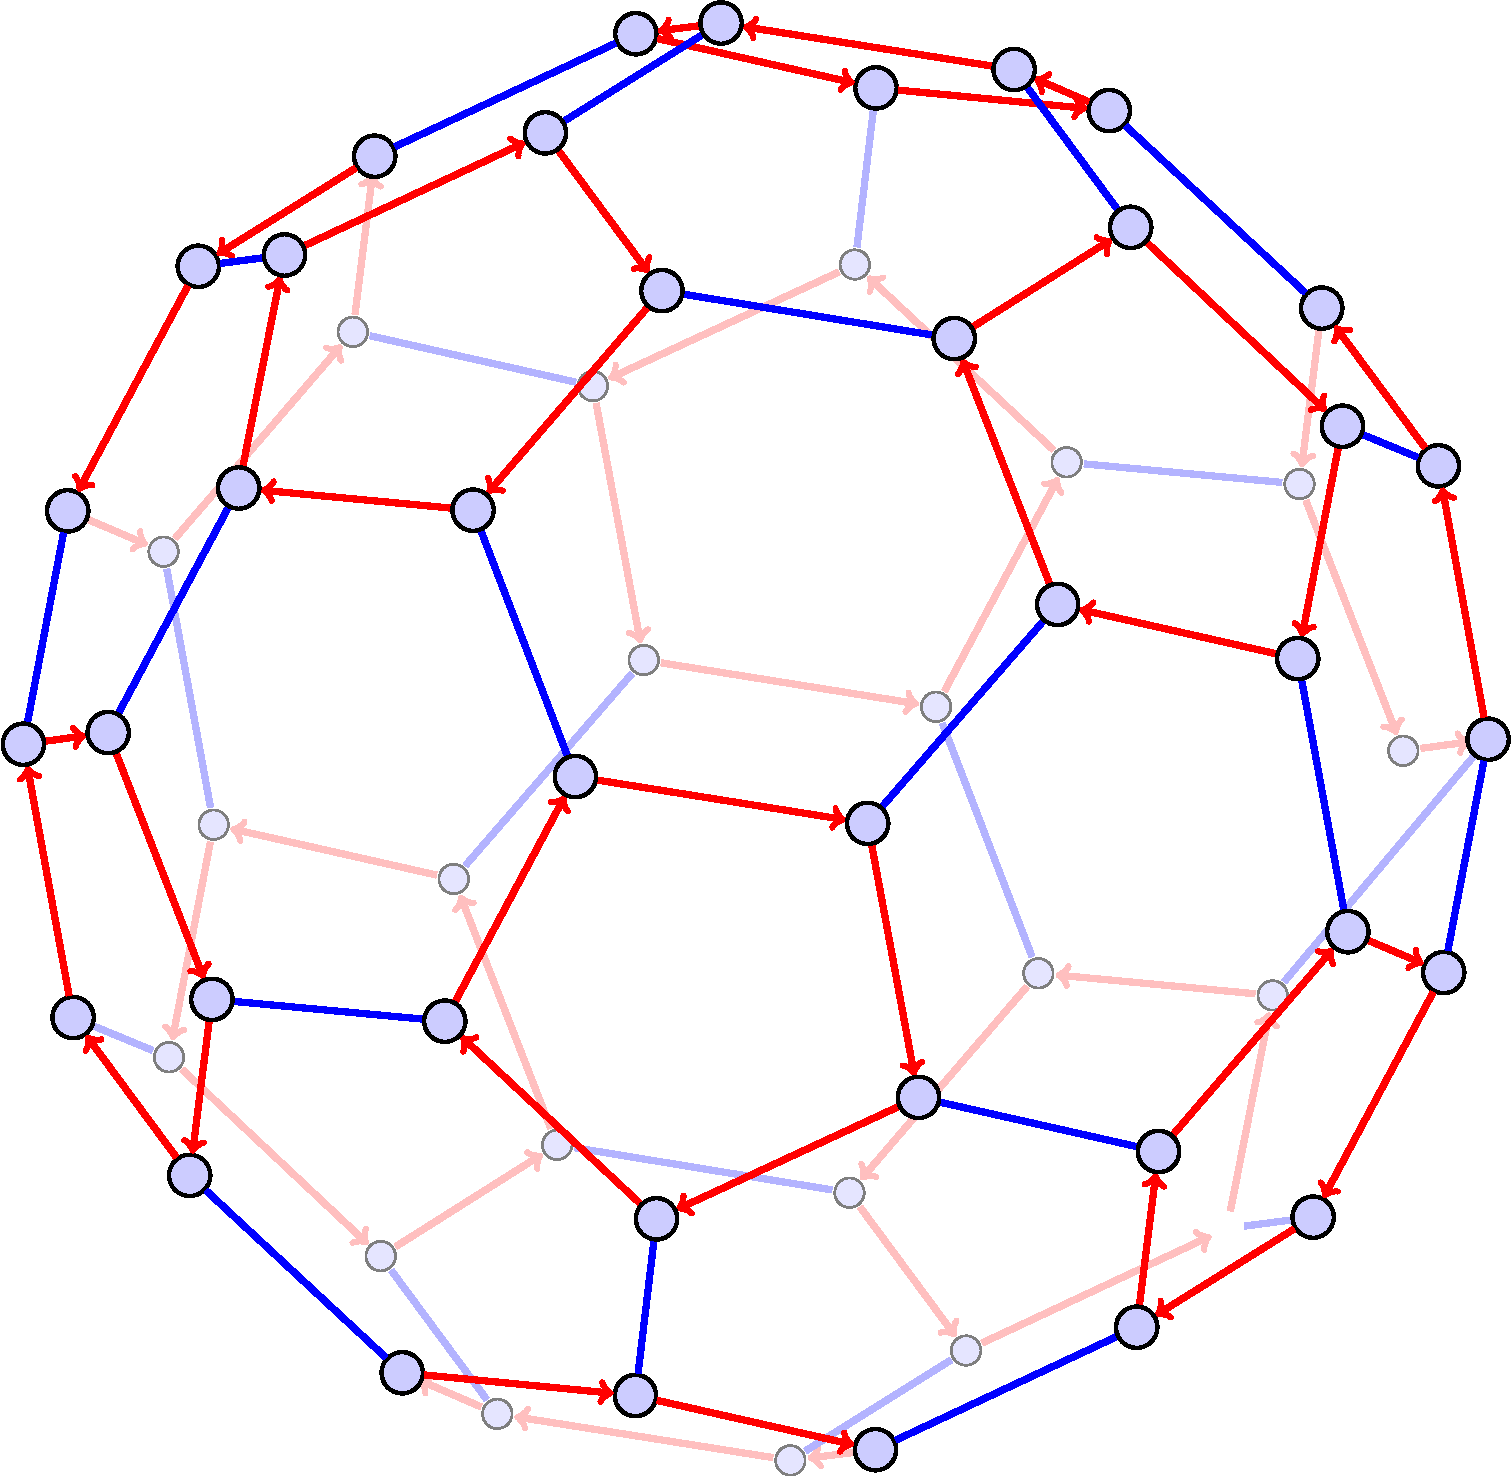
\includegraphics[height=2.5cm]{example/m2.pdf}}
\hspace{4em}
\subcaptionbox{PDF 图像,注意这个图略矮些。如果标题很长的话,它会自动换行\label{fig3}}
{	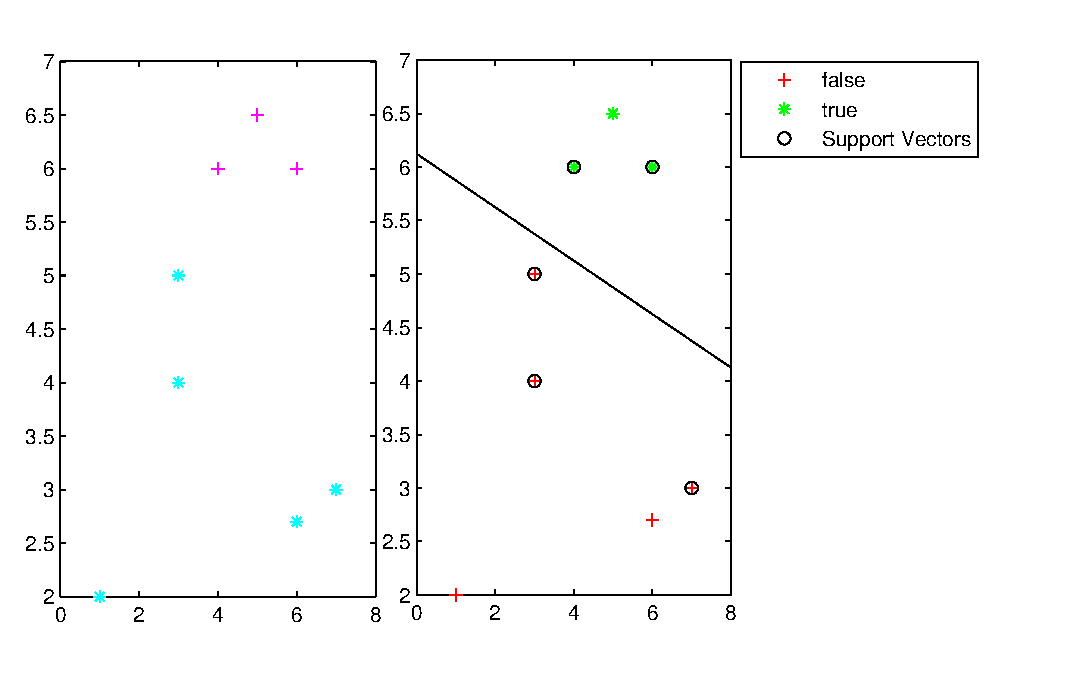
\includegraphics[scale=0.5]{example/figep.eps}}
\bicaption{插入eps和pdf的例子(使用 subcaptionbox 方式)}{An EPS and PDF demo with subcaptionbox}
\label{fig4}
\end{figure}




\section{插入代码}

这里给一个使用listings宏包插入源代码的例子:
\begin{lstlisting}[language={C}, caption={一段C源代码}]
#include <stdio.h>
#include <unistd.h>
#include <sys/types.h>
#include <sys/wait.h>

int main() {
pid_t pid;

switch ((pid = fork())) {
case -1:
printf("fork failed\n");
break;
case 0:
/* child calls exec */
execl("/bin/ls", "ls", "-l", (char*)0);
printf("execl failed\n");
break;
default:
/* parent uses wait to suspend execution until child finishes */
wait((int*)0);
printf("is completed\n");
break;
}

return 0;
}
\end{lstlisting}


\section{参考文献管理}
\label{sec2.5}
\LaTeX 具有将参考文献内容和表现形式分开管理的能力,涉及三个要素:参考文献数据库、参考文献引用格式、在正文中引用参考文献。
这样的流程需要多次编译:
\begin{enumerate}[noitemsep,topsep=0pt,parsep=0pt,partopsep=0pt]
\item 用户将论文中需要引用的参考文献条目,录入纯文本数据库文件(bib文件)。
\item 调用xelatex对论文模板做第一次编译,扫描文中引用的参考文献,生成参考文献入口文件(aux)文件。
\item 调用bibtex,以参考文献格式和入口文件为输入,生成格式化以后的参考文献条目文件(bib)。
\item 再次调用xelatex编译模板,将格式化以后的参考文献条目插入正文。
\end{enumerate}

参考文献数据库(thesis.bib)的条目,可以从Google Scholar搜索引擎\footnote{\url{https://scholar.google.com}}、CiteSeerX搜索引擎\footnote{\url{http://citeseerx.ist.psu.edu}}中查找,文献管理软件Papers\footnote{\url{http://papersapp.com}}、Mendeley\footnote{\url{http://www.mendeley.com}}、JabRef\footnote{\url{http://jabref.sourceforge.net}}也能够输出条目信息。

下面是在Google Scholar上搜索到的一条文献信息,格式是纯文本:

\begin{lstlisting}[caption={从Google Scholar找到的参考文献条目}, label=googlescholar, escapeinside="", numbers=none]
@phdthesis{"白2008信用风险传染模型和信用衍生品的定价",
title={"信用风险传染模型和信用衍生品的定价"},
author={"白云芬"},
year={2008},
school={"上海交通大学"}
} 
\end{lstlisting}

推荐修改后在bib文件中的内容为:

\begin{lstlisting}[caption={修改后的参考文献条目}, label=itemok, escapeinside="", numbers=none]
@phdthesis{bai2008,
title={"信用风险传染模型和信用衍生品的定价"},
author={"白云芬"},
date={2008},
address={"上海"},
school={"上海交通大学"}
} 
\end{lstlisting}

参考文献的引用:
\begin{itemize}
\item 参考文献在正文中被引用,使用命令\verb+\cite{key}+,如\cite{M91}。
\item 参考文献未引用但仍希望列在书末的参考文献中,使用命令\verb+\nocite{key}+,如\verb+\nocite{WI64,G03,D01,JS03}+.
\end{itemize}
\nocite{WI64,G03,D01,JS03}
% %# -*- coding: utf-8-unix -*-


% %# -*- coding: utf-8-unix -*-
%%==================================================

% \include{tex/chapter5}
% \include{tex/chapter6}
% \include{tex/chapter7}
% 


% \include{tex/chapter9}
% \include{tex/chapter10}
% \backmatter	
%======================================================================
% 打印参考文献
\printbibliography[heading=bibintoc]
\makeatletter
\makeatother
\end{document}